\chapter{Methodology}
\label{chap-four}
A methodology that incorporates the different sources of cumulative damage in RC structures is proposed. Different models of aging conditions that modify the material properties are studied, these are then incorporated into the analytical model.

The aging conditions focused on this research are:
\begin{itemize}
	\item Corrosion
	\item Strain aging
\end{itemize}

Other aging conditions, such as concrete strength aging, repairs, welding and fatigue in steel structures,  will be added later to this study.

\section{Modeling of corrosion for structural analysis}

Corrosion has been shown to modify the mechanical properties of stell, as discussed in section 2.1. These findings have been incorporated in the structural analysis at the material level. Results obtained from the experimental phase outlined in \ref{chap-three} will be incorporated in this analysis.The incorporation of corrosion in the analytical model is outlined as follows:
\begin{enumerate}
	\item The time for initiation of corrosion is calculated with equation \eref{eq.three} 
	\item The rate of corrosion is calculated according equation \eref{eq.CorrosionRate}
	\item The diameter of the rebar is reduced and the corrosion level is calculated using equations \eref{eq.CorrosionLevel} \eref{eq.CorrosionEvolution} 
	\item The mechanical properties of the reinforcing steel are modified with the corresponding corrosion level as shown in equation \eref{eq.eleven}
\end{enumerate}

This process is shown in \fref{fig:CorrModel}.

\begin{figure}[htbp]
	\centering
	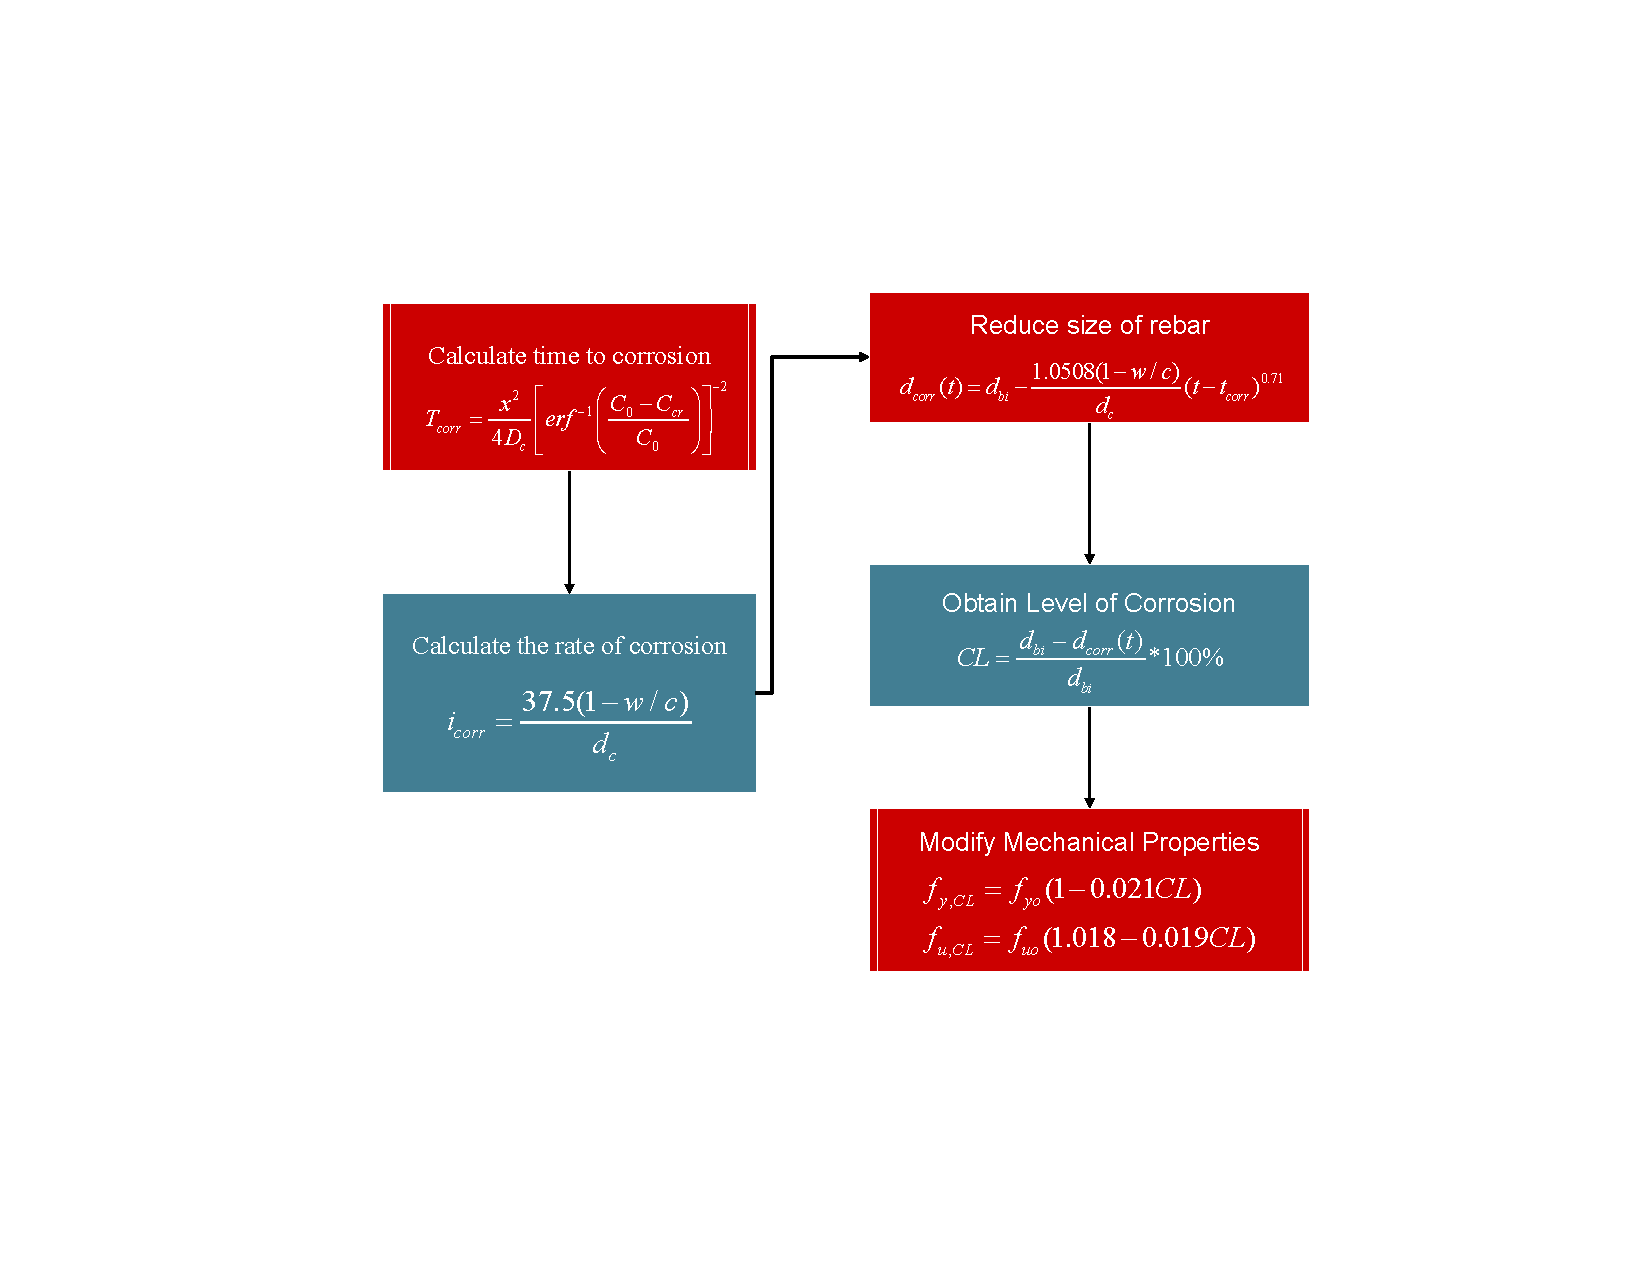
\includegraphics[width=0.7\textwidth]{Chapter-4/figs/Corrosion_Modeling}
	\caption{Corrosion modeling for structural analysis}
	\label{fig:CorrModel}
\end{figure}

This is later incorporated into the nonlinear structural analysis framework using OpenSeesPy \cite{McKenna2010}\cite{Zhu2018}, the framework of this analysis is explained in section 4.6.

\section{Modeling of strain aging for structural analysis}
In mild steel such as grade 60 reinforcing steel the phenomenon of strain aging is of importance. Summarizing the strain aging process described in section 2.2, mild steel after being subjected to high strain, and after time has passed, the yield strength of the steel increases and the fracture strain decreases. The increase in strength of steel is 

\section{Multiple seismic events}

The evaluation of multiple seismic events is a topic that has been scarcely studied, however their effects have been felt in numerous earthquake sequences such as the Christchurch 2010, Umbria-Marche Earthquake 1997 and the Puerto Rico Earthquakes 2020. The hypothesis is that accumulation of damage will restart in a smaller seismic event to achieve a prescribed limit state, similar to how corrosion and other aging phenomena might impact the intensity needed to achieve a future limit state. 

For this study it has been determined that not all damage in structures are dependent on multiple events but rather their condition when an event occurs as is the case for corrosion. Other damage related phenomenons such as strain aging depend on the loading history and are therefore dependent on the history of extreme loading events. It is therefore proposed to study corrosion on a discrete modeling of main shocks each independent of the other and to study the effect on strain aging by using a sequence of Main Shocks.

\subsection{Earthquake selection}

For this study the NGA2 West Database of earthquake records provided by the Pacific Earthquake and Engineering Research Insitute (PEER) \cite{Ancheta2014} is used. This database consists of 599 different earthquake events that characterize the ground motions on the west coast of the contiguous United States. The data was filtered according to the following criteria:

\begin{itemize}
	\item Must be an earthquake sequence
	\item Moment magnitude $M_w \geqslant 5$
	\item $PGA>0.04$
	\item $PGV>1$ cm/s
	\item $Vs_{30}>100m/s$ \& $Vs_{30}<1000$ m/s
	\item Lowest usable frequency is less than 1Hz
	\item $R_{rup}<60km$
\end{itemize}

From this data the main shocks found are the following earthquakes which can be summarized in \fref{fig:MS_Selection}. Figure \ref{fig:MS_Selection} shows the earthquakes as moment magnitude {Mw} vs rupture distance ($R_{rup}$).

\begin{itemize}
	\item Chi-chi
	\item Managua
	\item Livermore
	\item Northridge
	\item Duzce 
	\item Mammoth lake
\end{itemize}

\begin{figure}[htbp]
	\centering
	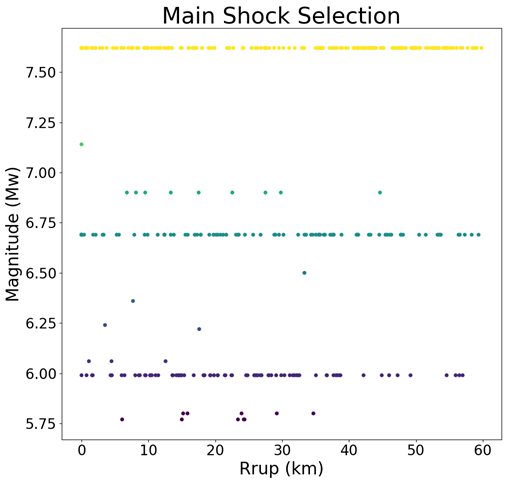
\includegraphics[width=0.6\textwidth]{Chapter-4/figs/MainShock_Selection}
	\caption{Mainshock selection from PEER NGA West2 database}
	\label{fig:MS_Selection}
\end{figure}

\subsection{Discrete modeling of main shock series}
The discrete modeling of mainshocks consists of using individual earthquakes that occur at different times throughout the life of the structures which correlate to a corrosion level (CL), this can be done for each of the main shocks selected after which the following data is obtained and later analyzed:

\begin{itemize}
	\item Maximum axial strain in confined concrete, cover and reinforcing steel 
Strains
	\item Obtain the probability of exceeding a given limit state $P(\varepsilon >\varepsilon_{LS},IM)$
	\item The earthquakes are characterized according to an intensity measure

\end{itemize}


\subsection{Multiple main shock series}

To simulate the life of a structure a mainshock series consisting of 3 mainshocks for a the life of a structure is considered, three phases are considered:
\begin{enumerate}

	\item At time $t=0$ the structure has pristine conditions
	\item Mainshock 1: pristine conditions are present. No changes to the material properties is present and no accumulation of damage has occurred.
	\item Mainshock 2: significant time after time to corrosion, mainshock 2 occurs and  material properties have changed due to corrosion
	\item Mainshock 3: corrosion and strain aging have occurred and further modified the properties of the materials.
\end{enumerate}

%This is shown graphically in \fref{fig:MSSequence}
%
%\begin{figure}[htbp]
%	\centering
%	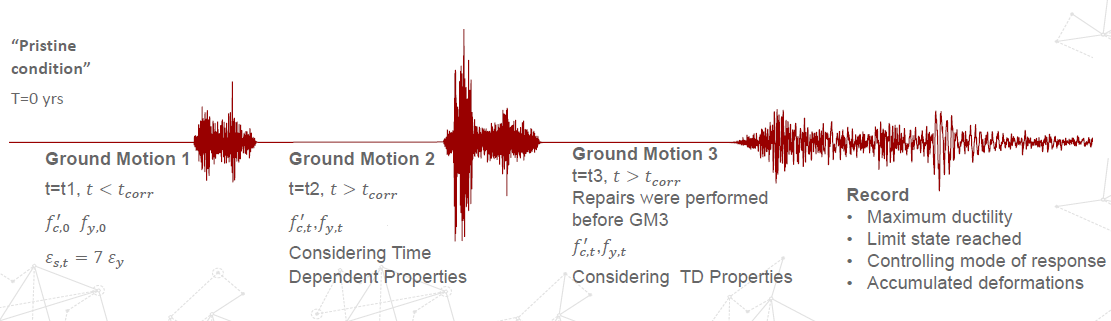
\includegraphics[width=0.9\textwidth]{Chapter-4/figs/MainShock_Sequence}
%	\caption{Mainshock sequence example}
%	\label{fig:MSSequence}
%\end{figure}

Similar to the discrete modeling of main shock series the following results can be obtained:

\begin{itemize}
	\item Maximum axial strain in confined concrete, cover and reinforcing steel 
Strains
	\item Obtain the probability of exceeding a given limit state $P(\varepsilon\varepsilon_{LS},IM)$
	\item The earthquakes are characterized according to an intensity measure

\end{itemize}

\section{Analytical Model}

\subsection{Cantilever column}
This study focuses on the behavior of a single degree of freedom (SDOF) system representing a cantilever reinforced concrete column. The column is modeled as shown in \fref{fig:Structural_Model} This structure is modeled in OpenSeesPy \cite{McKenna2010}\cite{Zhu2018} using the $forceBeamColumn$ element \cite{Scott}. The forceBeamColumn element is used with two-point Gauss-Radau integration applied in the hinge regions and two-point Gauss integration applied on the element interior for a total of six integration points \cite{Scott}. The force-based formulation requires only a single element to accurately represent the full nonlinear deformation of the member and the integration scheme selected prevents the loss of objectivity during softening response while also providing integration points at the member ends \cite{Calabrese2010},\cite{Scott}. The element requires the length of plasticity be defined at each end of the member, for which the tension-based rectangular plastic hinge length is calculated using the following expressions \cite{Goodnight2013}:

\begin{equation}
    L_{pc}=k*L_{eff} + 0.4D
    \label{eq:LP_Comp}
\end{equation}
\begin{equation}
	k=0.2*(Fu/Fy - 1) \leqslant 0.08
	\label{eq:K_Lp}
\end{equation}
\begin{equation}
    L_{pt}=L_{pc}+\gamma*D
    \label{eq:LP_Tension}
\end{equation}

For single bending the parameter $\gamma$ is:
\begin{equation}
    \gamma=0.33
    \label{eq:Gamma_LPt}
\end{equation}

The two-point Gauss-Radau integration is applied such that each end node integration is weighted equal to the specified plastic hinge length, as illustrated in \fref{fig:Fiber_PlasticHinge}. Therefore, strains recorded at the end sections represent accurate values even in the case where deformation localizes to the ends from strain-softening behavior. For the case of the cantilever column considered, only one plastic hinge length is defined, and the opposite end is given an arbitrary unit length. 

\begin{figure}[htbp]
	\centering
	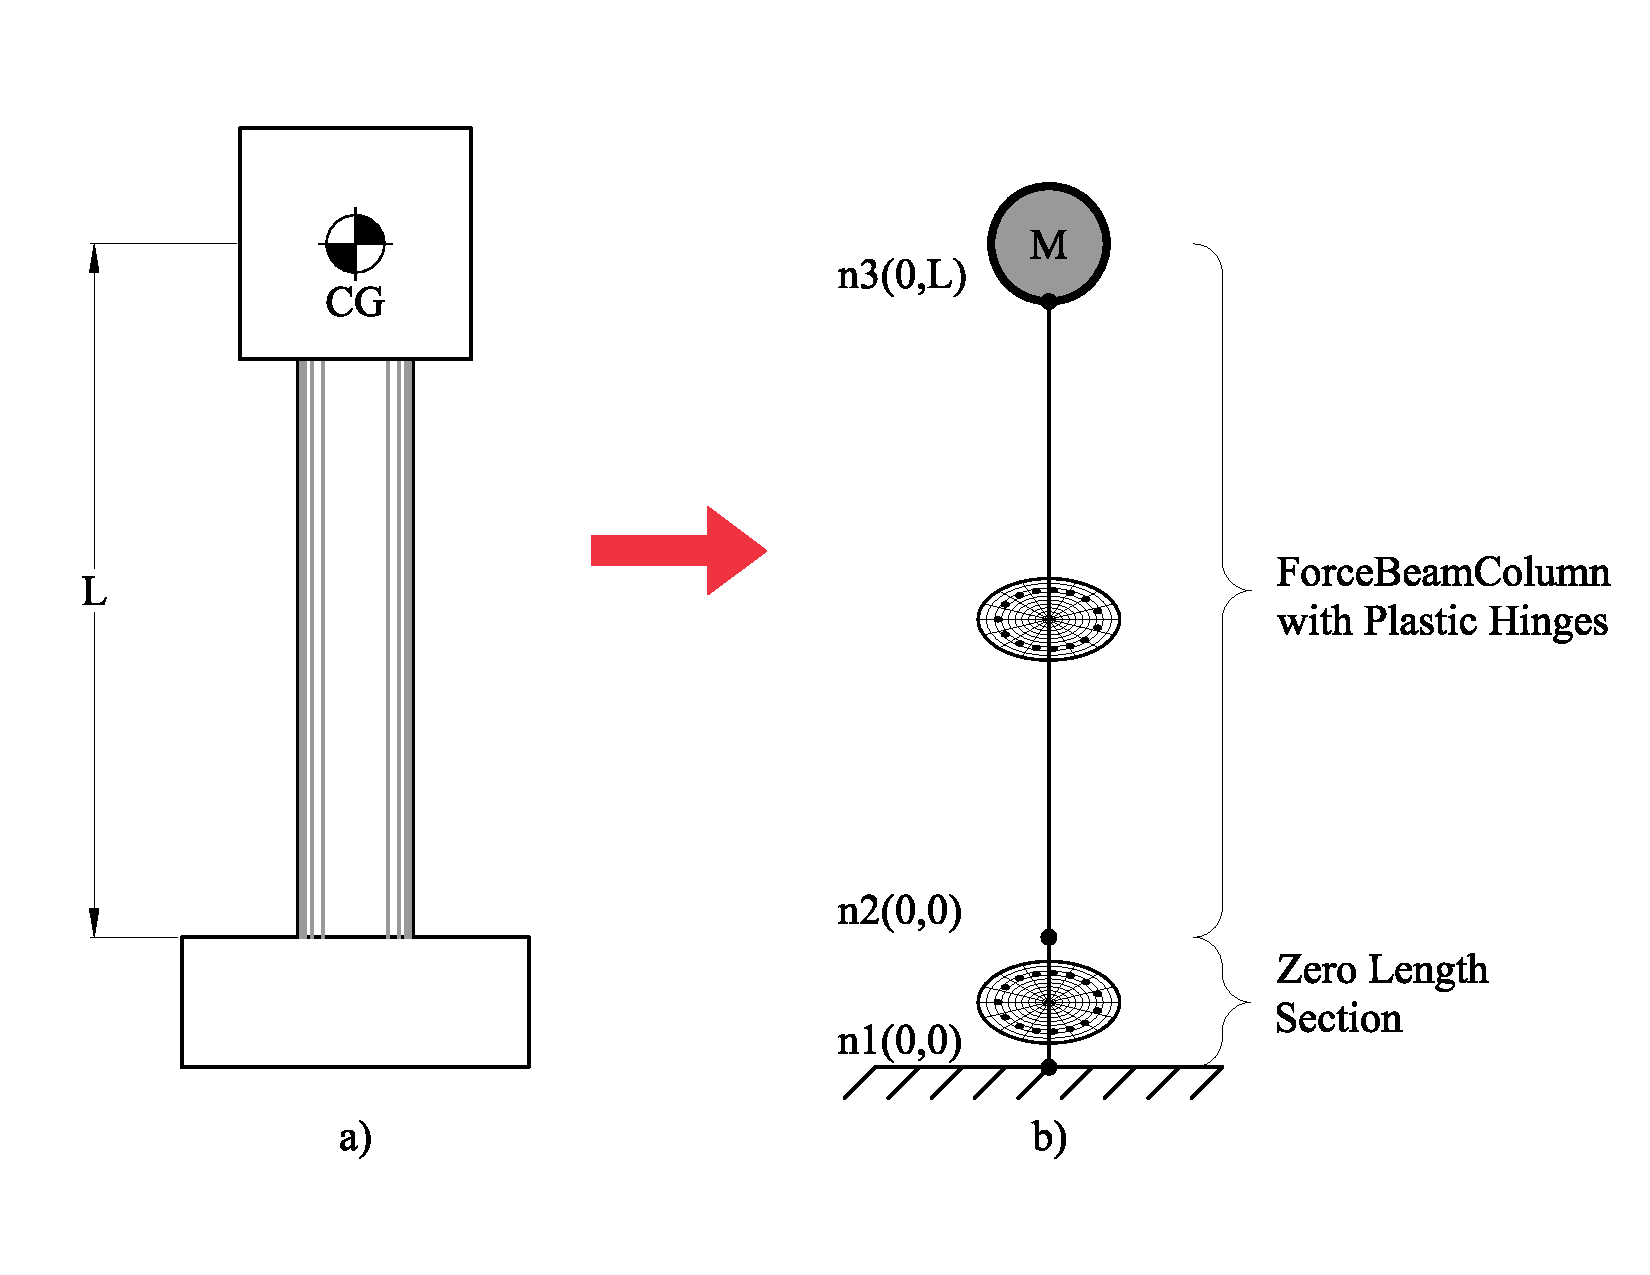
\includegraphics[width=0.75\textwidth]{Chapter-4/figs/StructuralModel_01}
	\caption{Structural Model a) SDOF Column b) Structural Model}
	\label{fig:Structural_Model}
\end{figure}

\begin{figure}[htbp]
	\centering
	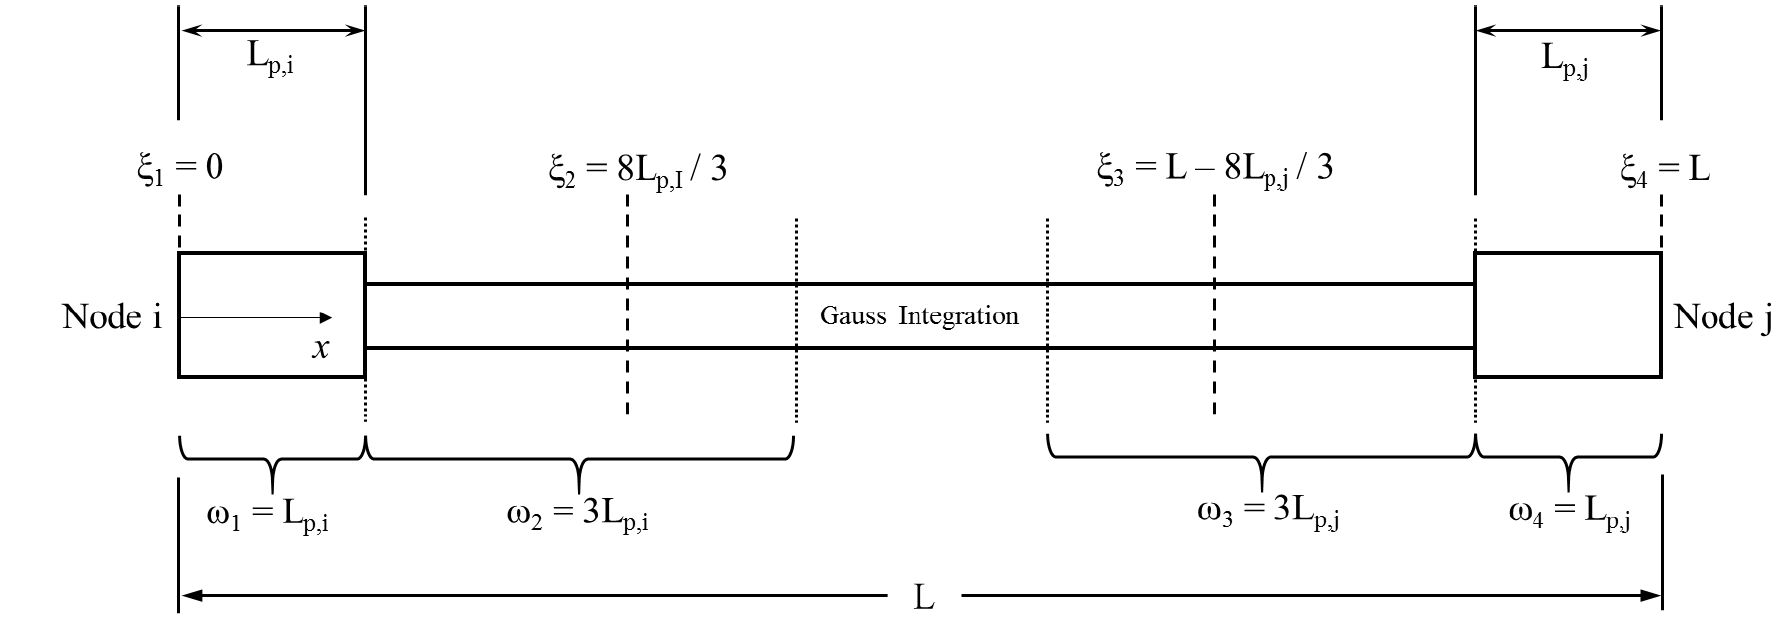
\includegraphics[width=0.9\textwidth]{Chapter-4/figs/fbc_PlasticHinge}
	\caption{End point plastic hinge method \cite{Scott}}
	\label{fig:Fiber_PlasticHinge}
\end{figure}

The section of the column is shown in \fref{fig:ColumnSection}, the section is discretized with concrete and steel material fibers. Concrete fibers are modeled using the $Concrete01$ material, modified for confined material strength based on the Mander confined concrete model \cite{Mander1988}. The $Steel02$ material, based on the Giuffre-Menegotto-Pinto model \cite{Filippou1983} is used for the longitudinal reinforcement with recommended parameters ($b = 0.01, R0 = 20, cR1 = 0.925, cR2 = 0.15$). 

\begin{figure}[htbp]
	\centering
	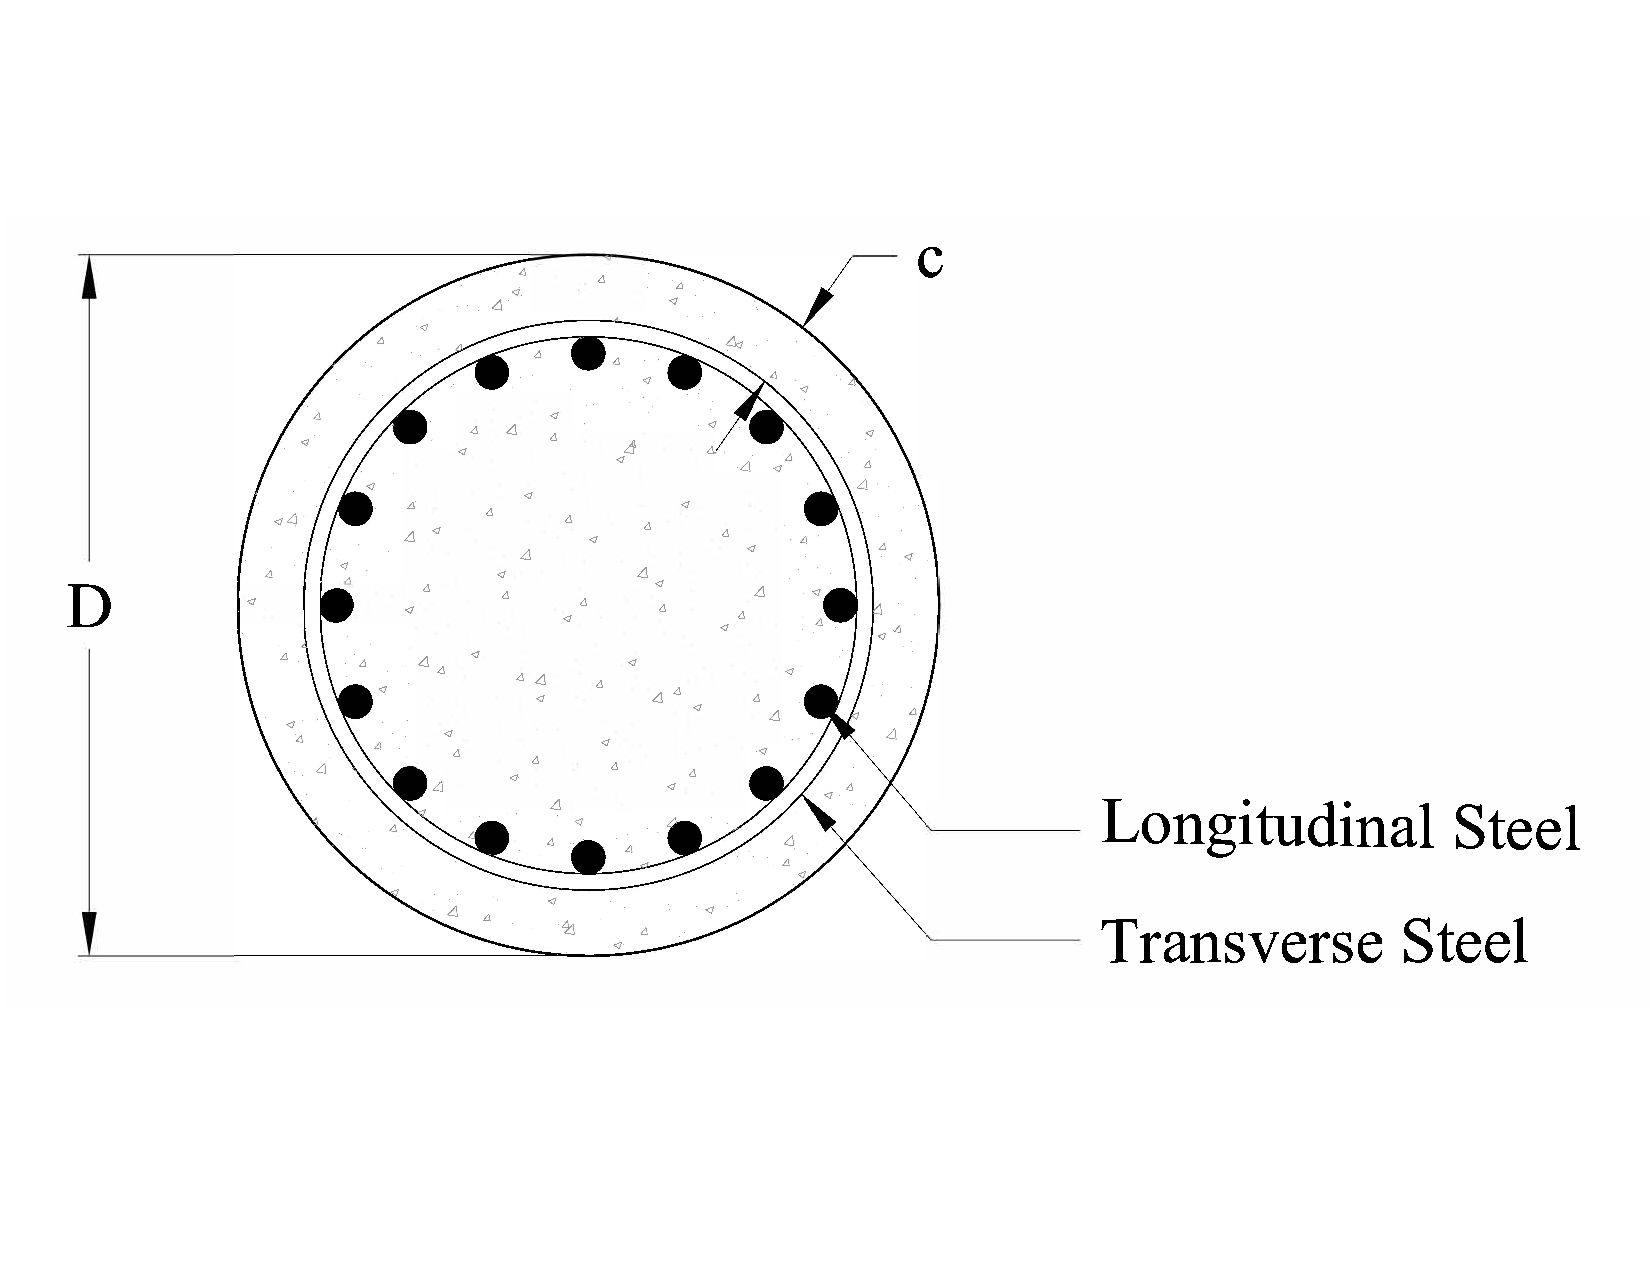
\includegraphics[width=0.7\textwidth]{Chapter-4/figs/StructuralModel_Section}
	\caption{Section of the RC Column}
	\label{fig:ColumnSection}
\end{figure}
\subsection{Strain penetration}

The strain penetration considers the additional deformation due to anchorage of the reinforcement into the foundation, since tension strain in the reinforcement will drop to zero at a depth equal to the true development length of the rebar \cite{Priestley2007}. Experimental studies have generally reported that this end rotation contributes up to 35\% to the lateral deformation of flexural members\cite{Zhao2007} and it is, therefore, important to incorporate into the analytical model. A way to capture this effect is by using a zero-length section element implemented in the nonlinear fiber-based analysis of concrete structures, this is available in the material library of OpenSeesPy as $Bond SP1$ \cite{Zhao2007} this is the material model used for the steel fibers of the zero-length section element.

The required parameters for this model are:
\begin{itemize}
	\item $F_{y}$ Yield strength of the reinforcement steel
	\item $S_{y}$ Rebar slip at member interface under yield stress (see \eref{eq.Rebar_Slip})
	\item $F_{u}$ Ultimate strength of the reinforcement steel
	\item $S_{u}$ Rebar slip at the loaded end at the bar fracture strength a value of $35 S_{y}$ is recommended \cite{Zhao2007}
	\item $b$ Initial hardening ratio in the monotonic slip vs. bar stress response $b=0.45$ is recommended \cite{Zhao2007}
	\item $R$ Pinching factor for the cyclic slip vs. bar response $R=1.01$ is recommended \cite{Zhao2007}
	\item $d_b$ Rebar diameter
	\item $f'c$ Concrete compressive strength of the adjoining connection member
	\item $\alpha$ Parameter used in the local bond-slip relation and can be taken as $\alpha=0.4$ in accordance with CEB-FIP Model Code 90 \cite{CEB1993}
\end{itemize}

Bar slip is calculated as:
\begin{equation}
	S_{y}(in)=0.1\left(\frac{d_{b}F_{y}}{4000\sqrt{f'_{c}}}\left(2\alpha+1\right)\right)^{\frac{1}{\alpha}}+0.013 (in)
	\label{eq.Rebar_Slip}
\end{equation}
\subsection{Design limit states}
Design limit states are defined based on strains in the material since they can more accurately represent the different performance levels of a structure. Structure limit states are defined for tension strains in the rebars or compression strains in the concrete core. The values recommended in typical performance-based design of reinforced concrete bridge columns are shown in Table  \ref{tab:DesignLimitStates}. The serviceability limit states correspond to the compression strain at which concrete cover begins to crush and the peak tension strain which results in residual crack widths of approximately 1 mm. These limits are generally accepted as nominal limit states for RC members. The compression limit state for damage control is defined by the expression shown in eq. \ref{eq:ec_DamageControl} and it refers to the compression strain in the confined concrete at which fracture of the transverse reinforcement confining the core occurs \cite{Priestley2007}. This equation is obtained using the strain-energy balance between that absorbed by the confined core concrete and the capacity of the confining steel. The tension damage control limit state is defined by the strain at the onset of buckling which can be expressed according to \ref{eq:es_DamageControl}, this equation demonstrated accurate predictions of the onset of bar buckling on physical tests in SDOF Concrete Column \cite{Goodnight2016}. The bar buckling limit state could change as a result of the experimental campaign proposed in Chapter 4.

\begin{equation}
    \varepsilon_{c,spiral yield}=0.009-0.3\frac{A_{st}}{A_{g}} +3.9\frac{f_{yhe}}{E_{s}}
    \label{eq:ec_DamageControl}
\end{equation}

\begin{equation}
    \varepsilon_{s,BB}=0.03+700\rho_{s}  \frac{f_{yhe}}{E_{s}} -0.1\frac{P}{f'_{c}A_{g}}
    \label{eq:es_DamageControl}
\end{equation}


\begin{table}[htbp]
	\caption{Design limit states}
	\label{tab:DesignLimitStates}
	\centering	
		\begin{tabular}{|l|c|c|}
		\hline
		\cellcolor[HTML]{CC0000}{\color[HTML]{FFFFFF}Limit State} & \cellcolor[HTML]{CC0000}{\color[HTML]{FFFFFF}Concrete Limit State $\varepsilon_{c} (in/in)$} & \cellcolor[HTML]{CC0000}{\color[HTML]{FFFFFF}Reinforcing Steel Limit State $\varepsilon_{s} (in/in)$}\\  \hline	
		Serviciability       & 0.004                           & 0.015  \\  \hline	
		Damage Control       & Eq. \ref{eq:ec_DamageControl}   & Eq. \ref{eq:es_DamageControl}\\  \hline
		\end{tabular}
\end{table}
 
\section{Comparison with existing physical tests}
\subsection{Pristine condition columns}

Goodnight et al performed a total of 30 circular RC columns quasi-static tests to evaluate strain limit states \cite{Goodnight2016}. From this set of tests, a sample of one was taken to calibrate the analytical model. The test performed by Goodnight et al on an SDOF cantilever column shows similar geometry to that presented in \fref{fig:Fiber_PlasticHinge}. The parameters used in this large scale test were:

\begin{itemize}
	\item Diameter $D = 24.0 inch$
	\item Height of the column $L = 8.0 ft$
	\item Yield strength of steel $f_{y} = 574.0 MPa$
	\item Ultimate strength of steel $f_{u} = 753.3 * MPa$
	\item Longitudinal steel volumetric ratio $\rho_{s} = 1.5\% $
	\item Transverse steel volumetric ratio $\rho_{v} = 1.0\% $
	\item Strength of concrete at 8 days $f'_{c} = 39.8 MPa$
\end{itemize}

The analytical model utilized these parameters to compare the results from the model to the experimental results. The results from the analysis show good agreement with the experimental results as evidenced in \fref{fig:ModelCalibration}. This assures that the results obtained from the model predict the overall system behavior and can be used to analyze other configurations of the structural model.

\begin{figure}[htbp]
	\centering
	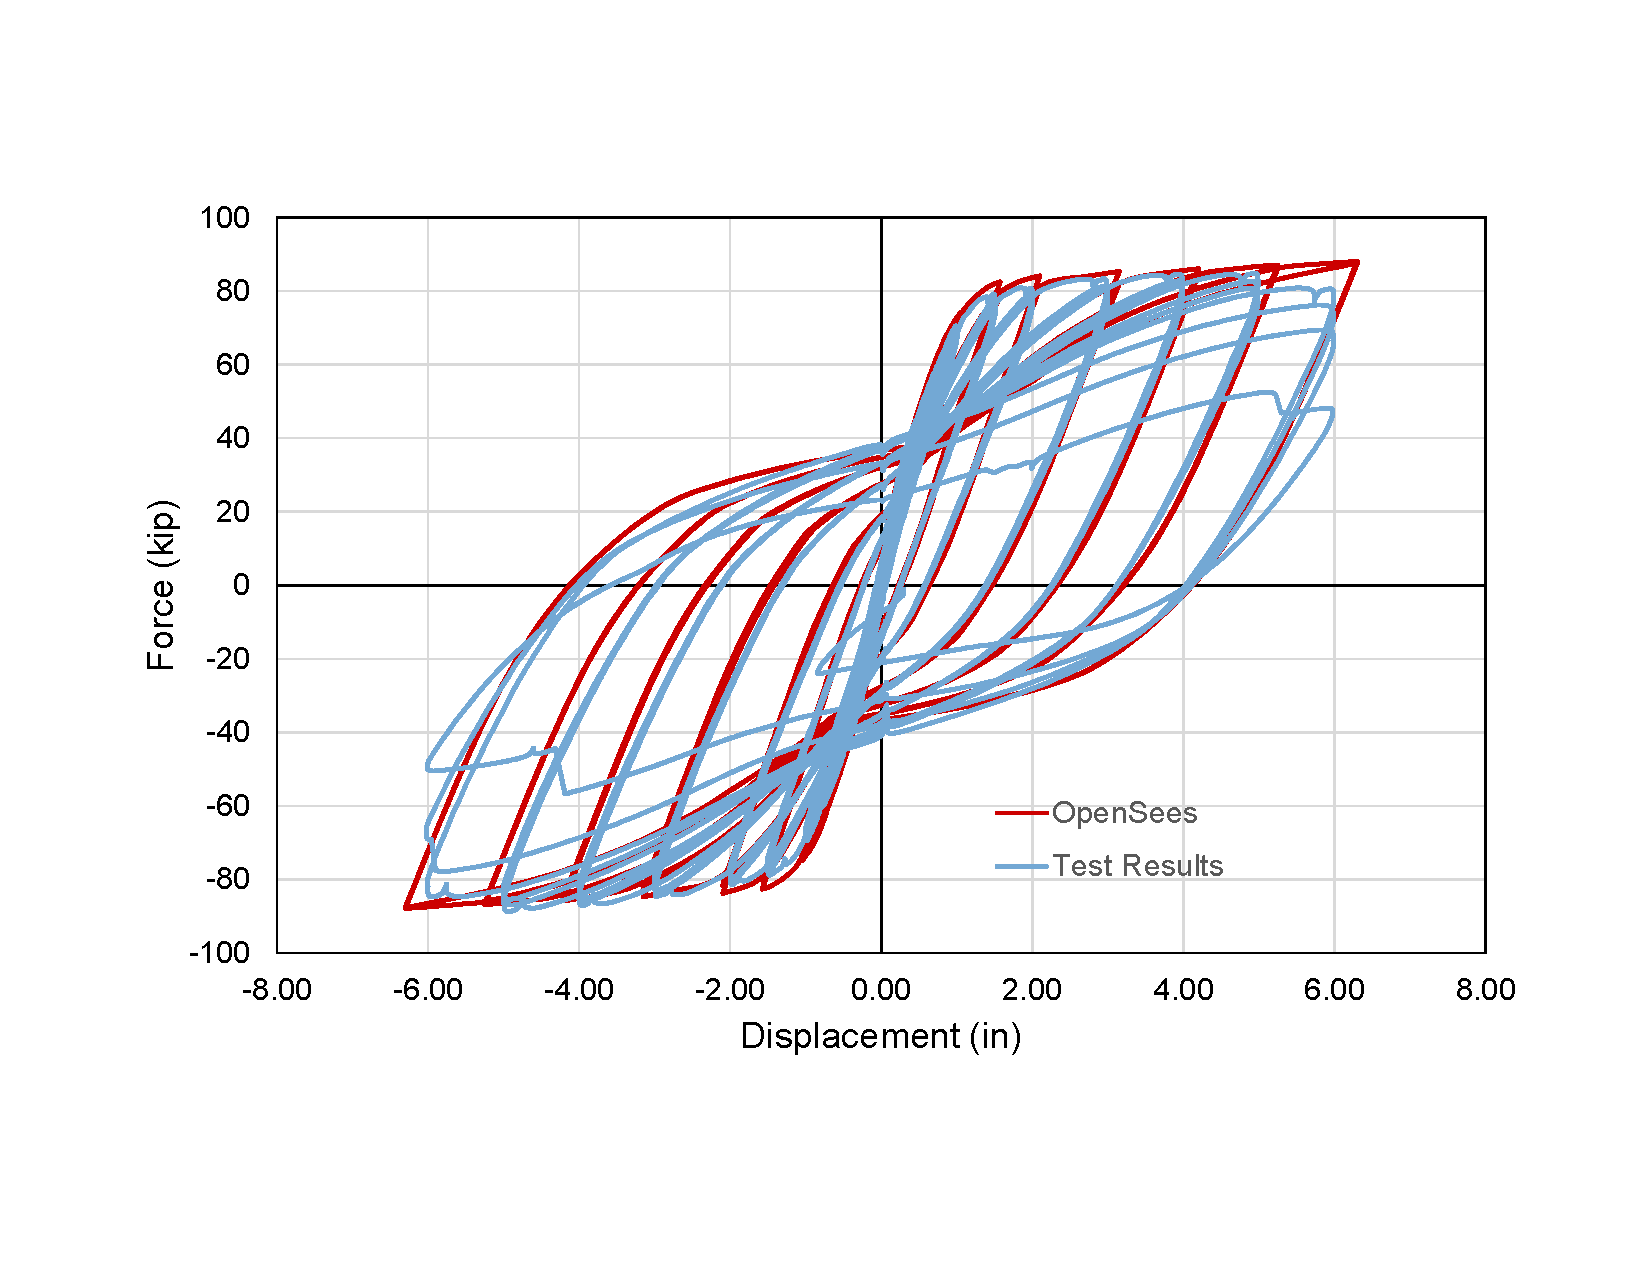
\includegraphics[width=0.7\textwidth]{Chapter-4/figs/Model_Calibration_Goodnight2016}
	\caption{Force-Displacement results from experimental results \cite{Goodnight2013} and analytical model}
	\label{fig:ModelCalibration}
\end{figure}
\subsection{Accelerated corrosion columns}
Similarly, Ma et al performed a series of quasi-static tests on RC columns with different corrosion levels and axial load ratios \cite{Ma2012}. From their study, the test with a corrosion level $CL=9.5\%$ was taken for calibration since the other tests presented in their study had excessively high axial load ratios which are not common in RC bridges. The results from Ma et al test	\cite{Ma2012} were used to compare against the analytical model. The column had the following parameters:
\begin{itemize}
	\item Diameter $D = 260.0 mm$
	\item Height of the column $L = 820.0 mm$
	\item Yield strength of steel $f_{y} = 375.0$ MPa
	\item Ultimate strength of steel $f_{u} = 572.3$ MPa
	\item Longitudinal steel volumetric ratio $\rho_{s} = 1.5\% $
	\item Transverse steel volumetric ratio $\rho_{v} = 1.0\% $
	\item Strength of concrete at 8 days $f'_{c} = 39.8$ MPa
	\item Corrosion level $CL=9.5\%$
\end{itemize}

In the analysis equation \eref{eq.eleven} is used to modify the material properties of the reinforcing steel, to consider the effects of corrosion. Figure \ref{fig:ModelCalibration_Corrosion} shows that the results obtained from the analytical model capture the response of the structure with some accuracy. Ma et al \cite{Ma2012} did not report if bar buckling and bar fracture occurred during the test. However, the hysteresis curve shown in their study suggests that some damage limit state was reached. To corroborate this, equation \eref{eq:es_DamageControl} is used to determine the bar buckling limit state ($\varepsilon_{s,BB}=0.024$), this is then compared to the analytical model results shown in figure \fref{fig:ModelCalibration_Corrosion_Hysteresis}. The results show a peak tension strain of $\varepsilon_{s}=0.023$. This result is close to the value obtained using equation \eref{eq:es_DamageControl}, thus pointing out the likelihood that the bar buckling limit state was observed during this test. While these results are close, it is still not clear if equation \eref{eq:es_DamageControl} captures the behavior of the buckling limit state for corroded rebars, therefore, the proposed corroded BBT test will show if corrosion affects the behavior of buckled bars.

\begin{figure}[htbp]
	\centering
	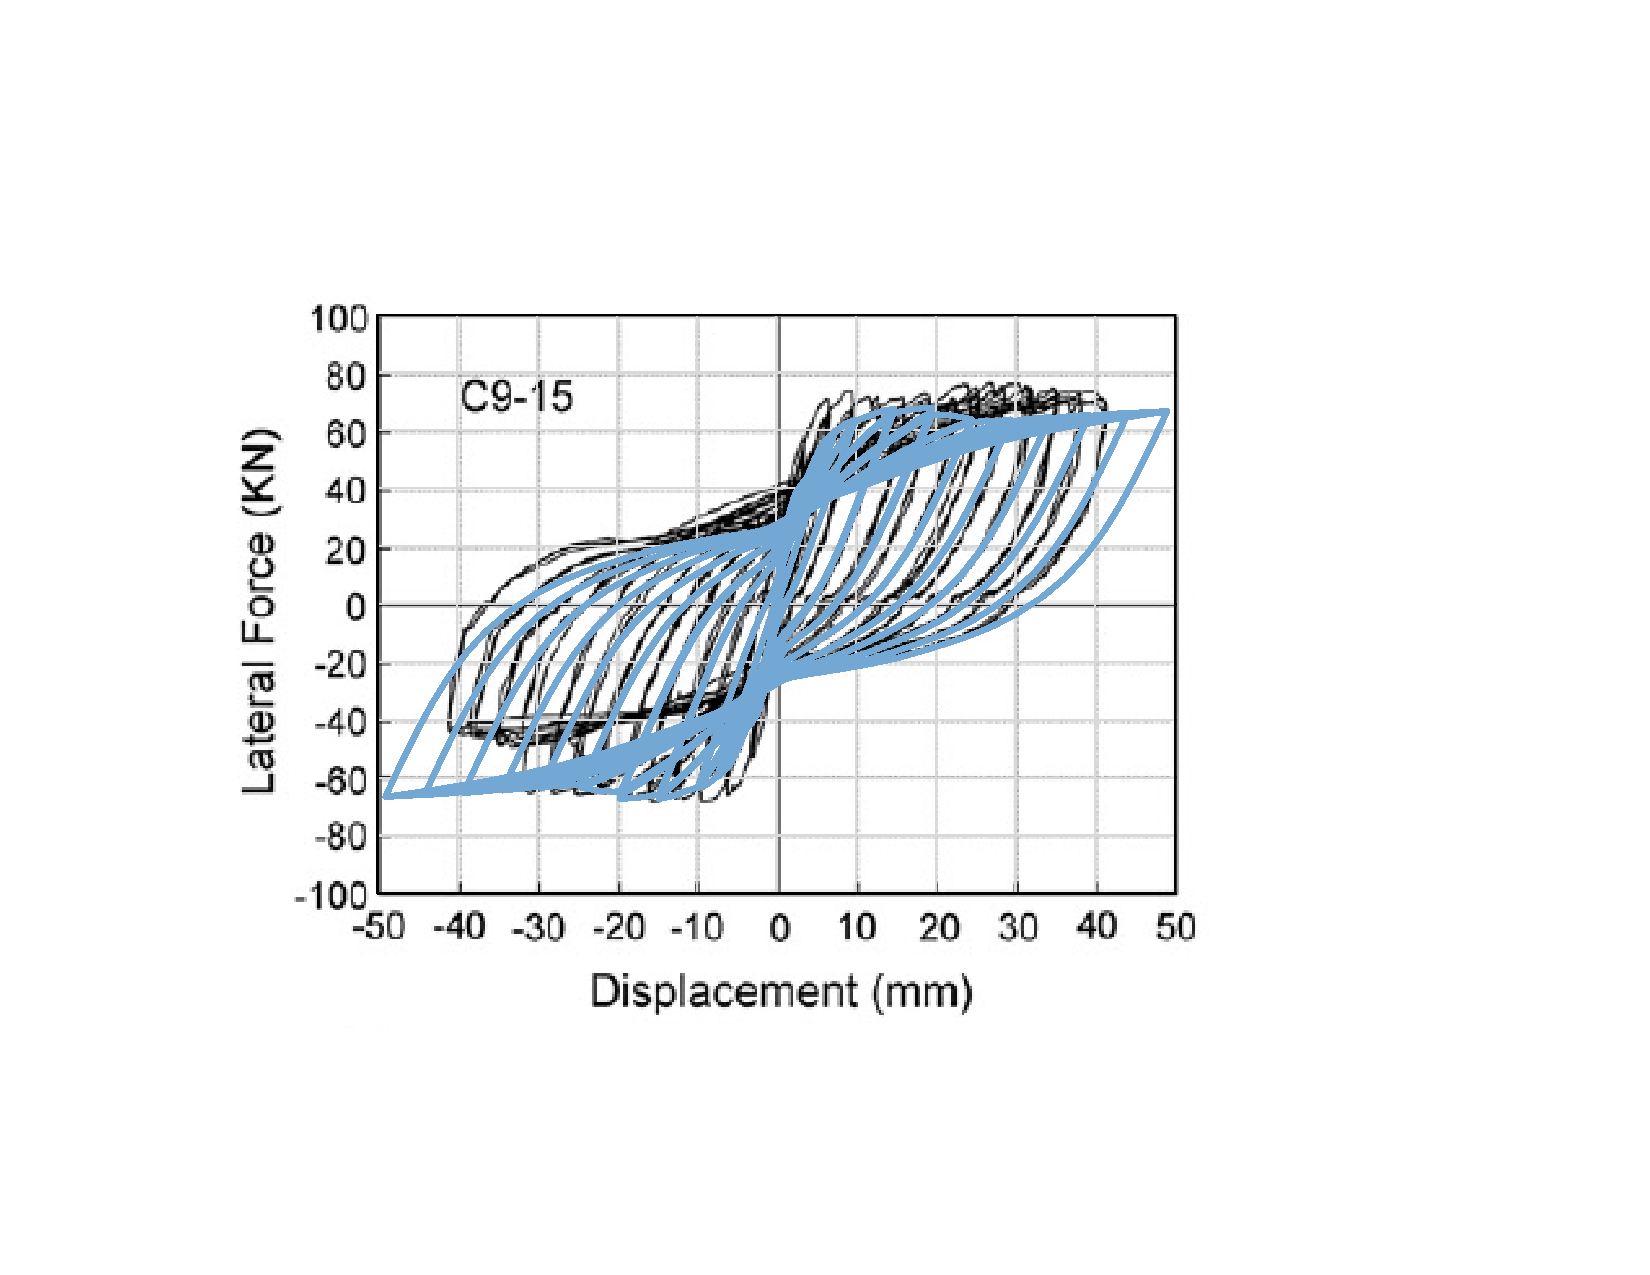
\includegraphics[width=0.7\textwidth]{Chapter-4/figs/Model_Calibration_Ma2012}
	\caption{Force-Displacement results from experimental RC column with corrosion in logitudinal bar (CL=9.5\%) results \cite{Ma2012} and analytical model (shown in lightblue)}
	\label{fig:ModelCalibration_Corrosion}
\end{figure}
\begin{figure}[htbp]
	\centering
	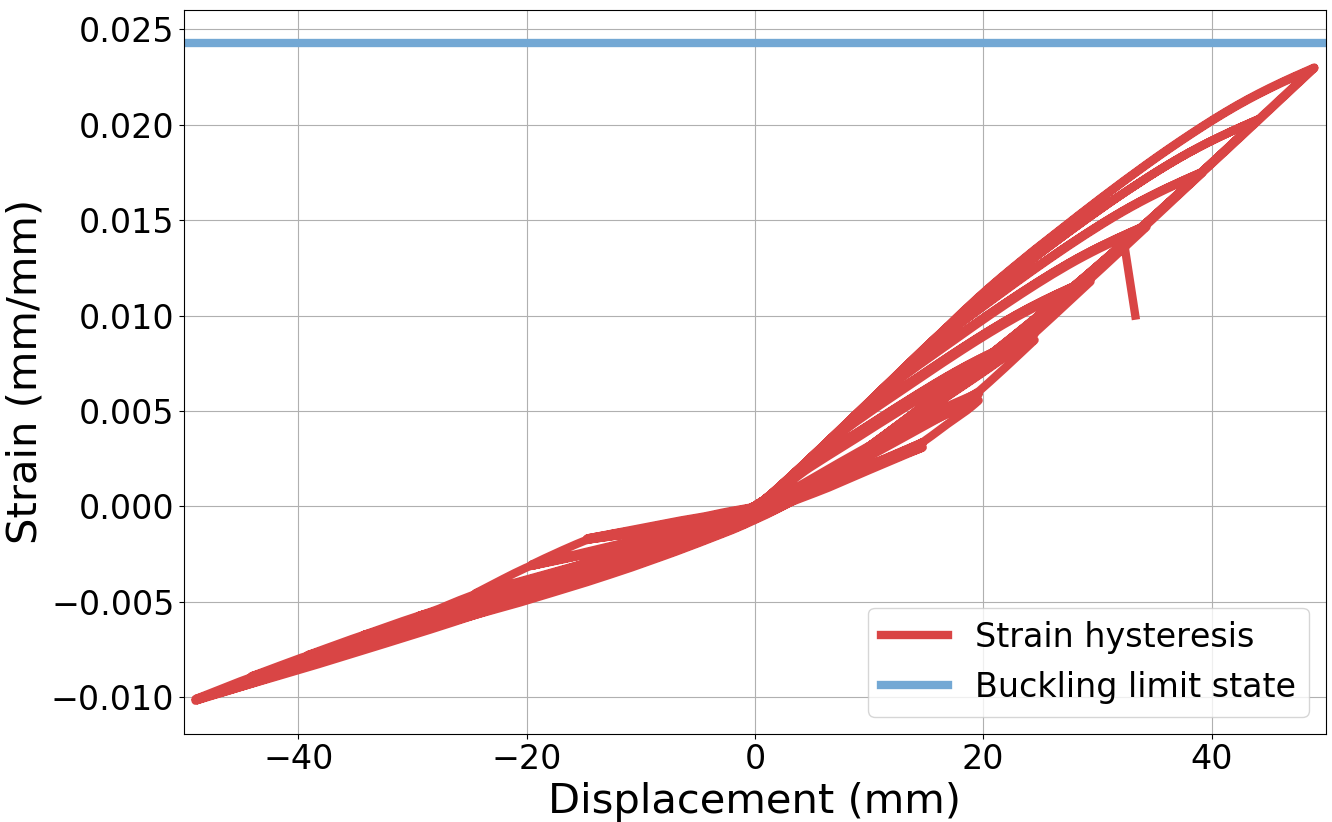
\includegraphics[width=0.9\textwidth]{Chapter-4/figs/MaEtAl_StrainHisteresis}
	\caption{Strain hysteresis from experimental RC column with corrosion in logitudinal bar (CL=9.5\%) results from analytical model}
	\label{fig:ModelCalibration_Corrosion_Hysteresis}
\end{figure}
\newpage

\section{Analytical framework}

An analytical framework is established to obtain the change in the structure performance due to aging conditions and evaluate the effect of multiple seismic events. Therefore, a series of nonlinear time history analyses (NLTHA) will be performed. From these analyses, it is possible to determine the effects of damage in the performance of structures. The proposed analytical framework process consists of:

\begin{enumerate}
	\item Geometrical properties of the SDOF column 
	\item Properties of the material are evaluated (i.e. water to cement ratio, cover)
	\item For equal periods of time the time dependent properties are modified
	\item Nonlinear time history analyses are performed for discrete ground motions or sequence of ground motions
	\item Results are obtained and evaluated
\end{enumerate}

The analysis matrix for the corrosion aging phenomenon that will be analyzed in this study is shown in Table \ref{tab:AnalysisMatrix}. The area or extent covered in the analysis corresponds to the range of variables that are common for RC columns in bridges.

\begin{table}[htb]
	\caption{Analysis matrix}
	\label{tab:AnalysisMatrix}
	\centering
\begin{tabular}{{|l|c|c|}}
\multicolumn{3}{c}{\cellcolor[HTML]{C90000}{\color[HTML]{FFFFFF} ANALYSIS MATRIX}} \\	\hline
Description                            & Parameter        & Range                  \\	\hline
Diameter of Column                     & D                & 30-90 in               \\	\hline
Column Length to Diameter Ratio        & L/D              & 2-8                    \\	\hline
Longitudinal Ratio                     & $\rho_s$         & 0.01-0.04              \\	\hline
Transverse Volumetric Ratio            & $\rho_v$         & 0.005-0.015            \\	\hline
Axial Load Ratio                       & ALR              & 0.05-0.2               \\	\hline
water to cement ratio                  & w/c              & 0.36-0.6               \\	\hline
cover                                  & c                & 1.5-3 in               \\	\hline
Time/Condition                         & CL               & 5\%-20\%               \\	\hline
\end{tabular}
\end{table}

%This procedure has been summarized in the form of a flow chart presented in \fref{fig:NLTHA_Framework}
%
%\begin{figure}[htbp]
%	\centering
%	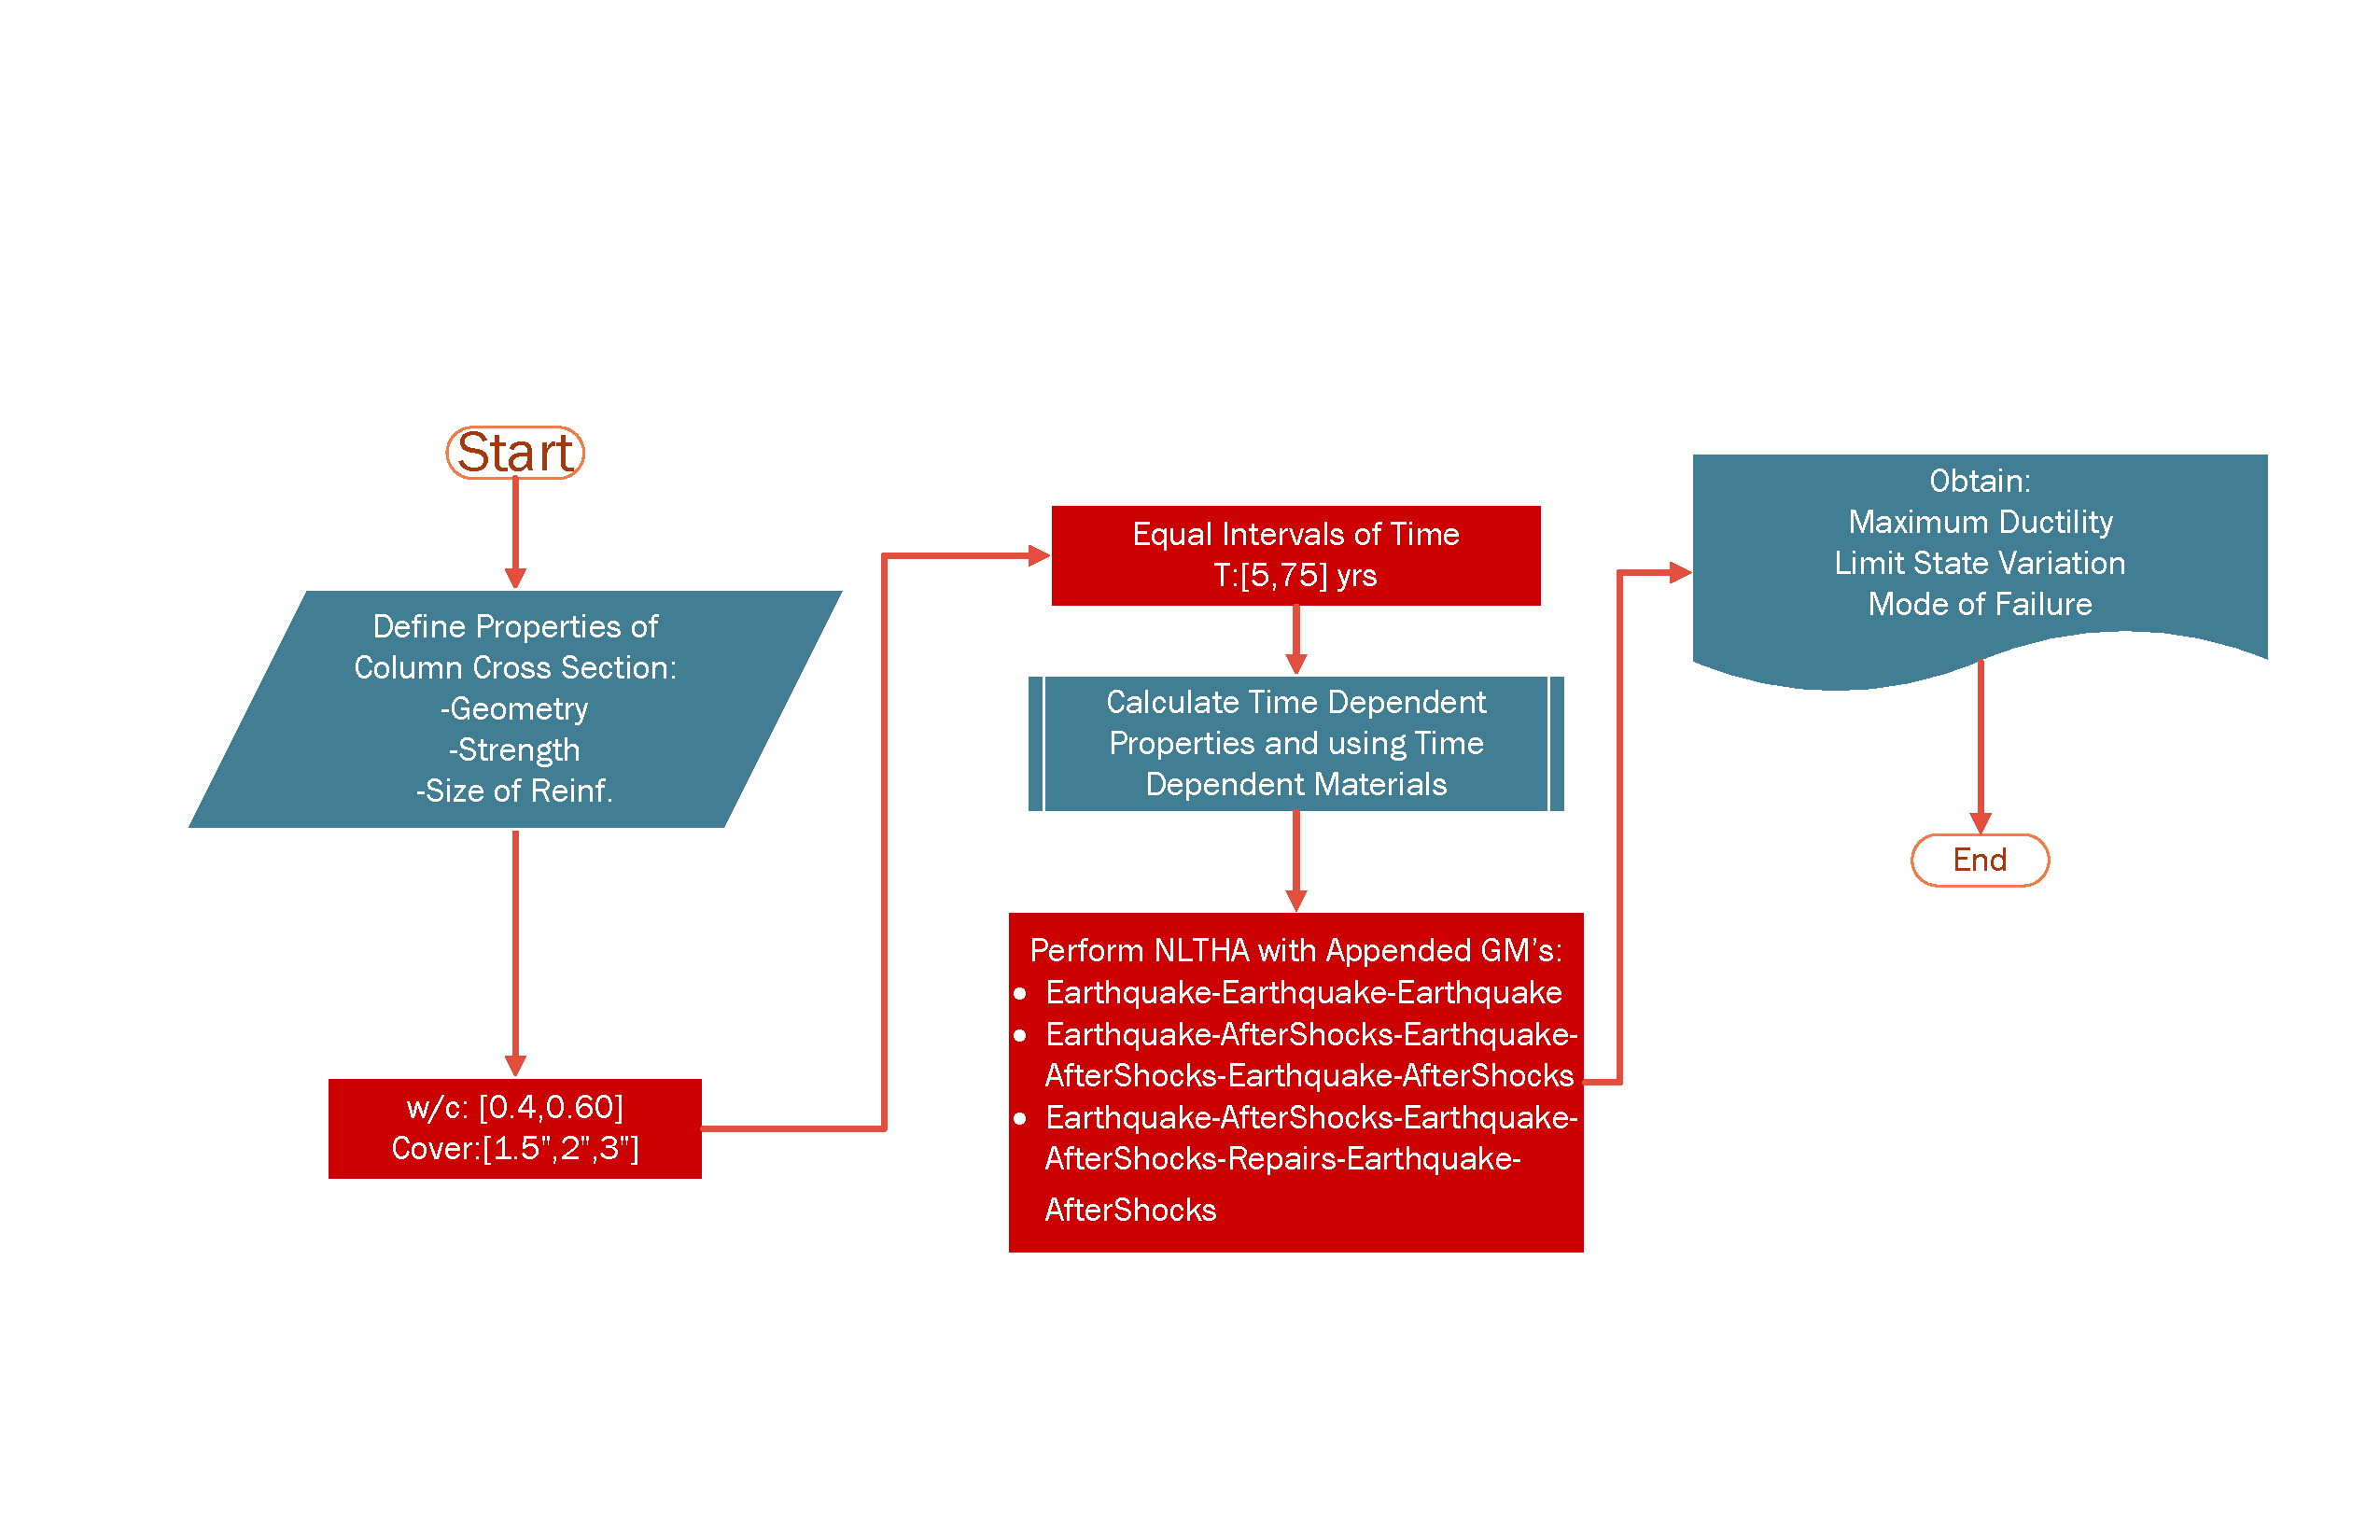
\includegraphics[width=0.9\textwidth]{Chapter-4/figs/AnalysisFramework_01}
%	\caption{Analysis Framework Flowchart}
%	\label{fig:NLTHA_Framework}
%\end{figure}
%
%\section{Earthquake selection}
%\lipsum[4]
\section{Results from NLTHA}
This section presents the results obtained from a non-linear time history analysis (NLTHA) performed using OpenSeesPy \cite{Zhu2018}. The structure was subjected to a total of 18 earthquake records. The main responses obtained from these analyses correspond to the maximum strain obtained for the different levels of corrosion. 

The structure used for this results currently corresponds to the parameters shown in section 5.2.1. The structure was analyzed for a range of corrosion levels [1.5\%-13\%] in the longitudinal rebars.

\subsection{Effect on structure response}
An example of the results obtained using NLTHA, figures \fref{fig:Force-Displacement_Results} and \fref{fig:Steel_Stress_Strain_Response} are presented. These results are extracted from the response of the structure to the Chi-Chi earthquake. \fref{fig:Force-Displacement_Results} shows the global system response and \fref{fig:Steel_Stress_Strain_Response} shows the stress-strain response of the extreme fiber of reinforcing steel. These results show that as corrosion increases the demands imposed on the structure increases too. Therefore an increase in the probability of reaching a limit state increases as corrosion increases.

\begin{figure}[htbp]
	\centering
	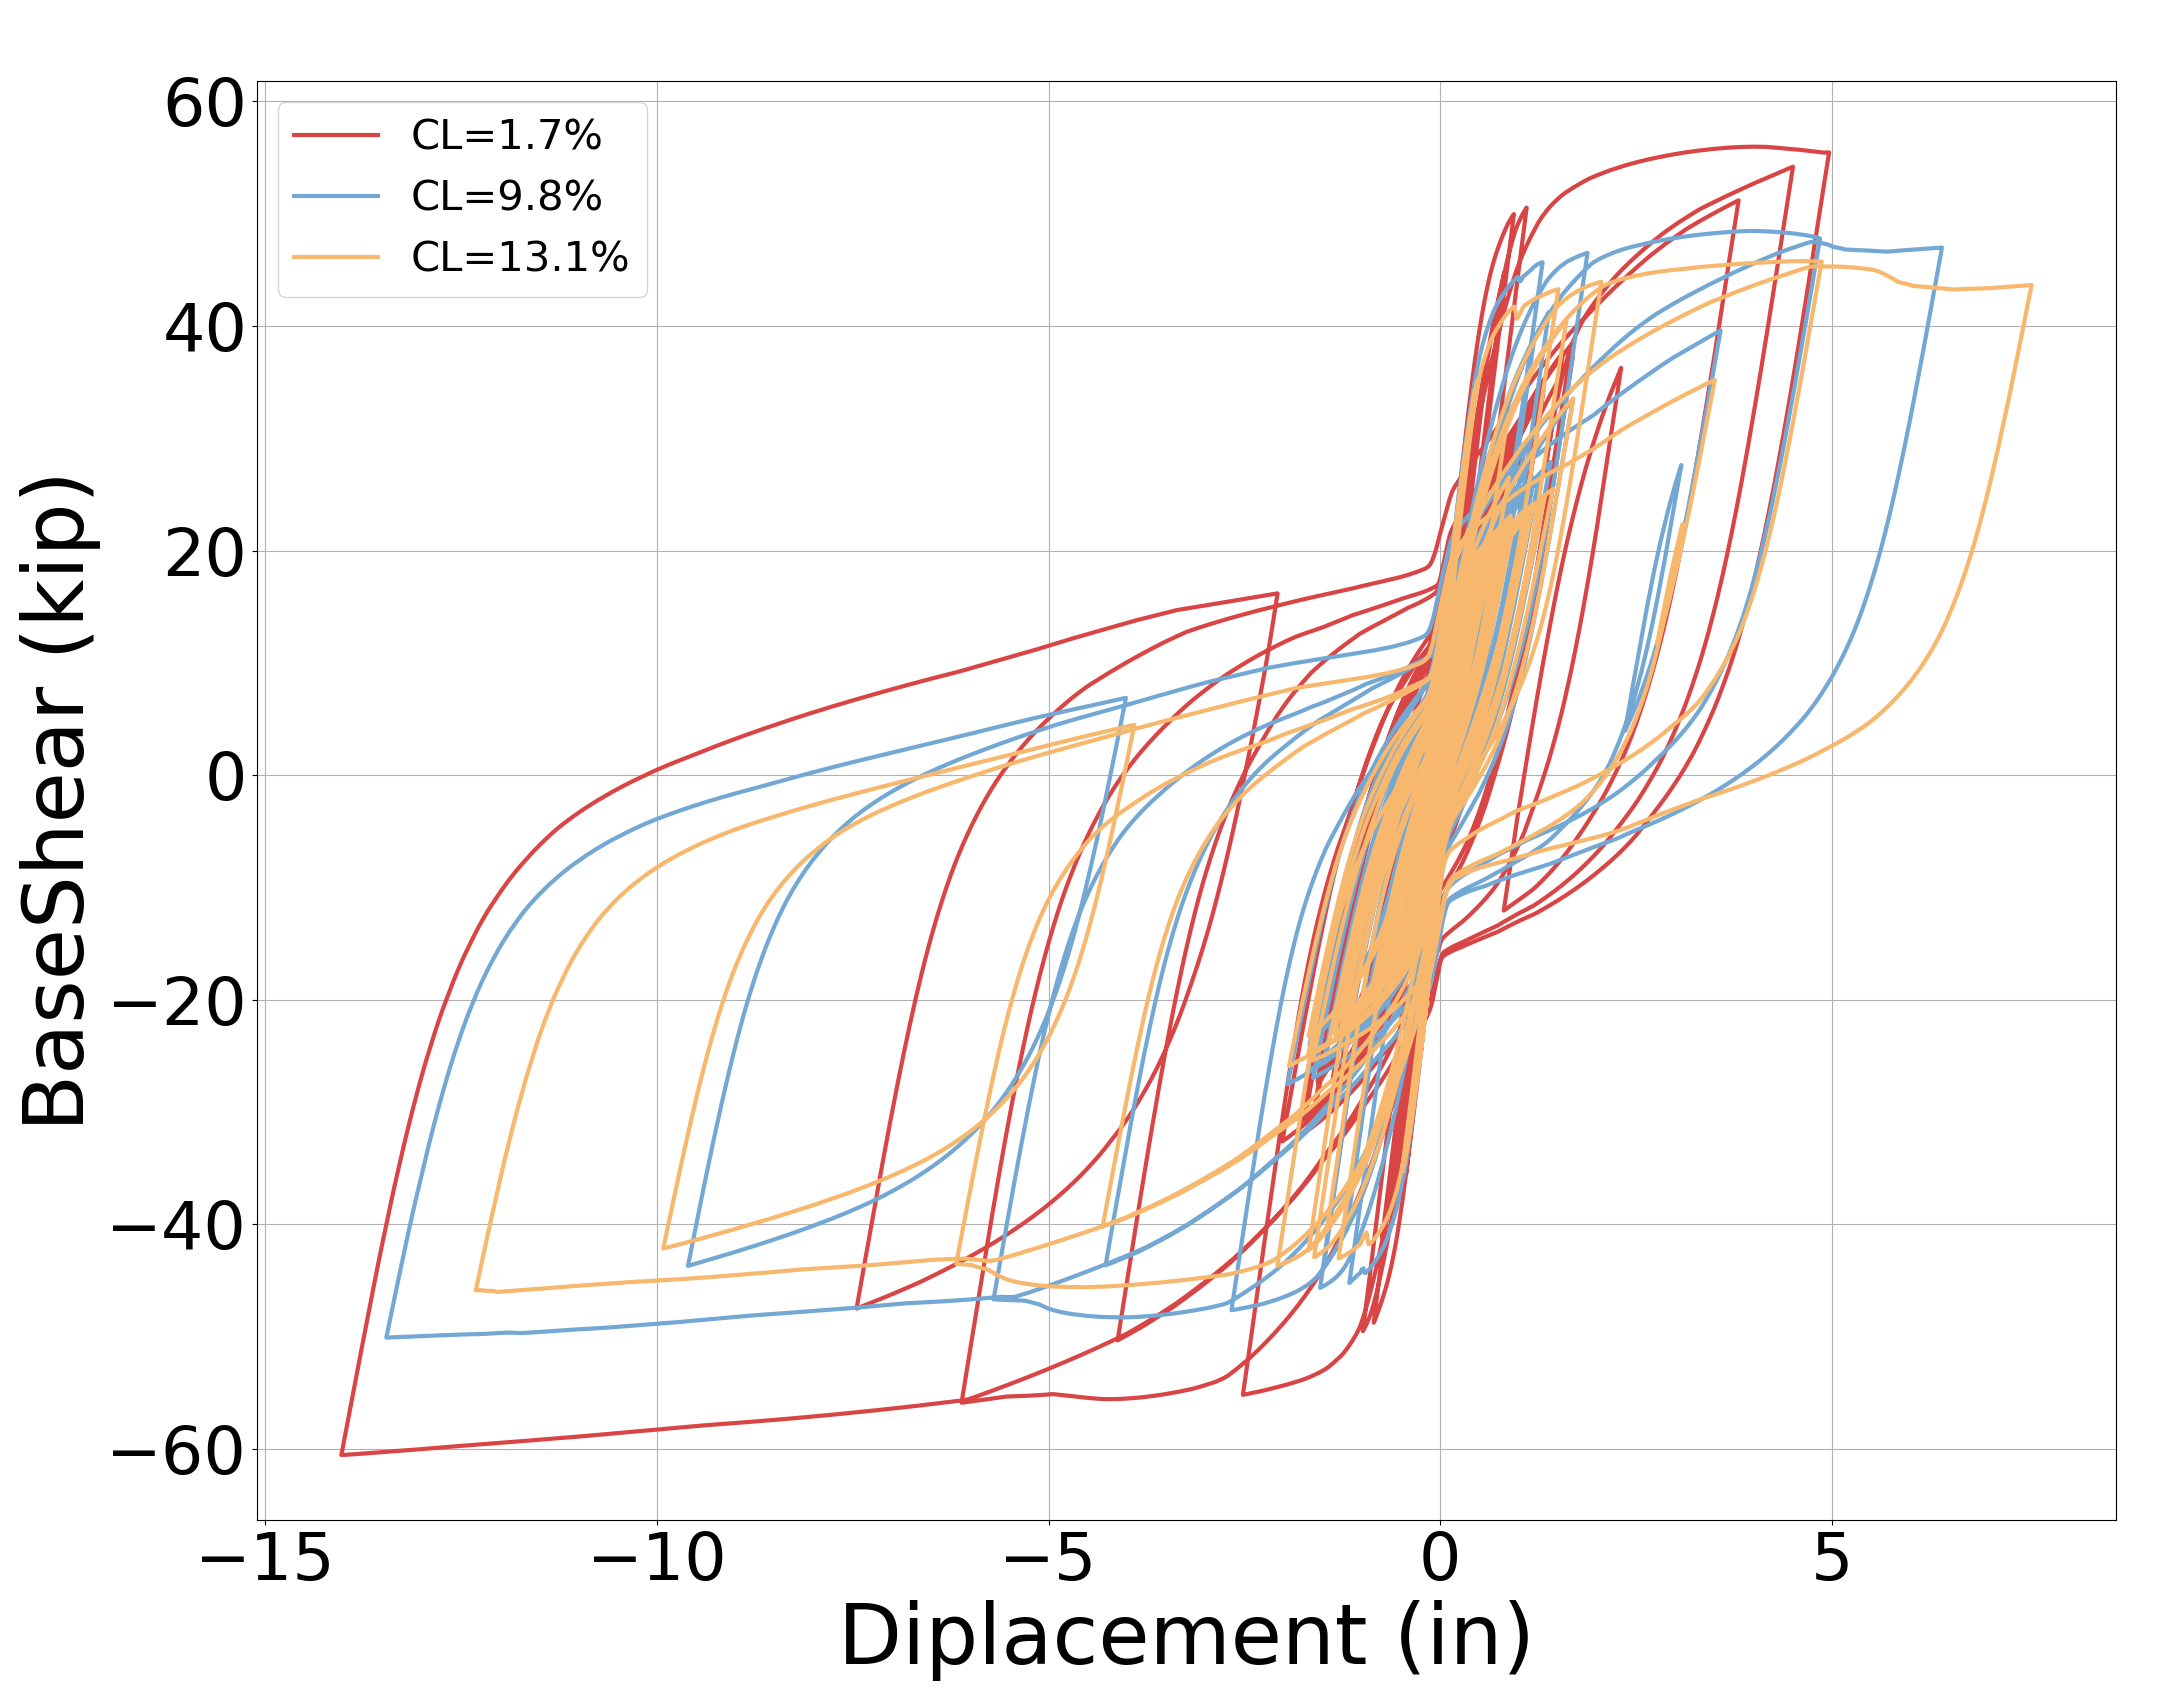
\includegraphics[width=0.65\textwidth]{Chapter-4/figs/ForceDisplacement_01}
	\caption{Force-Displacement results}
	\label{fig:Force-Displacement_Results}
\end{figure}
\begin{figure}[htbp]
	\centering
	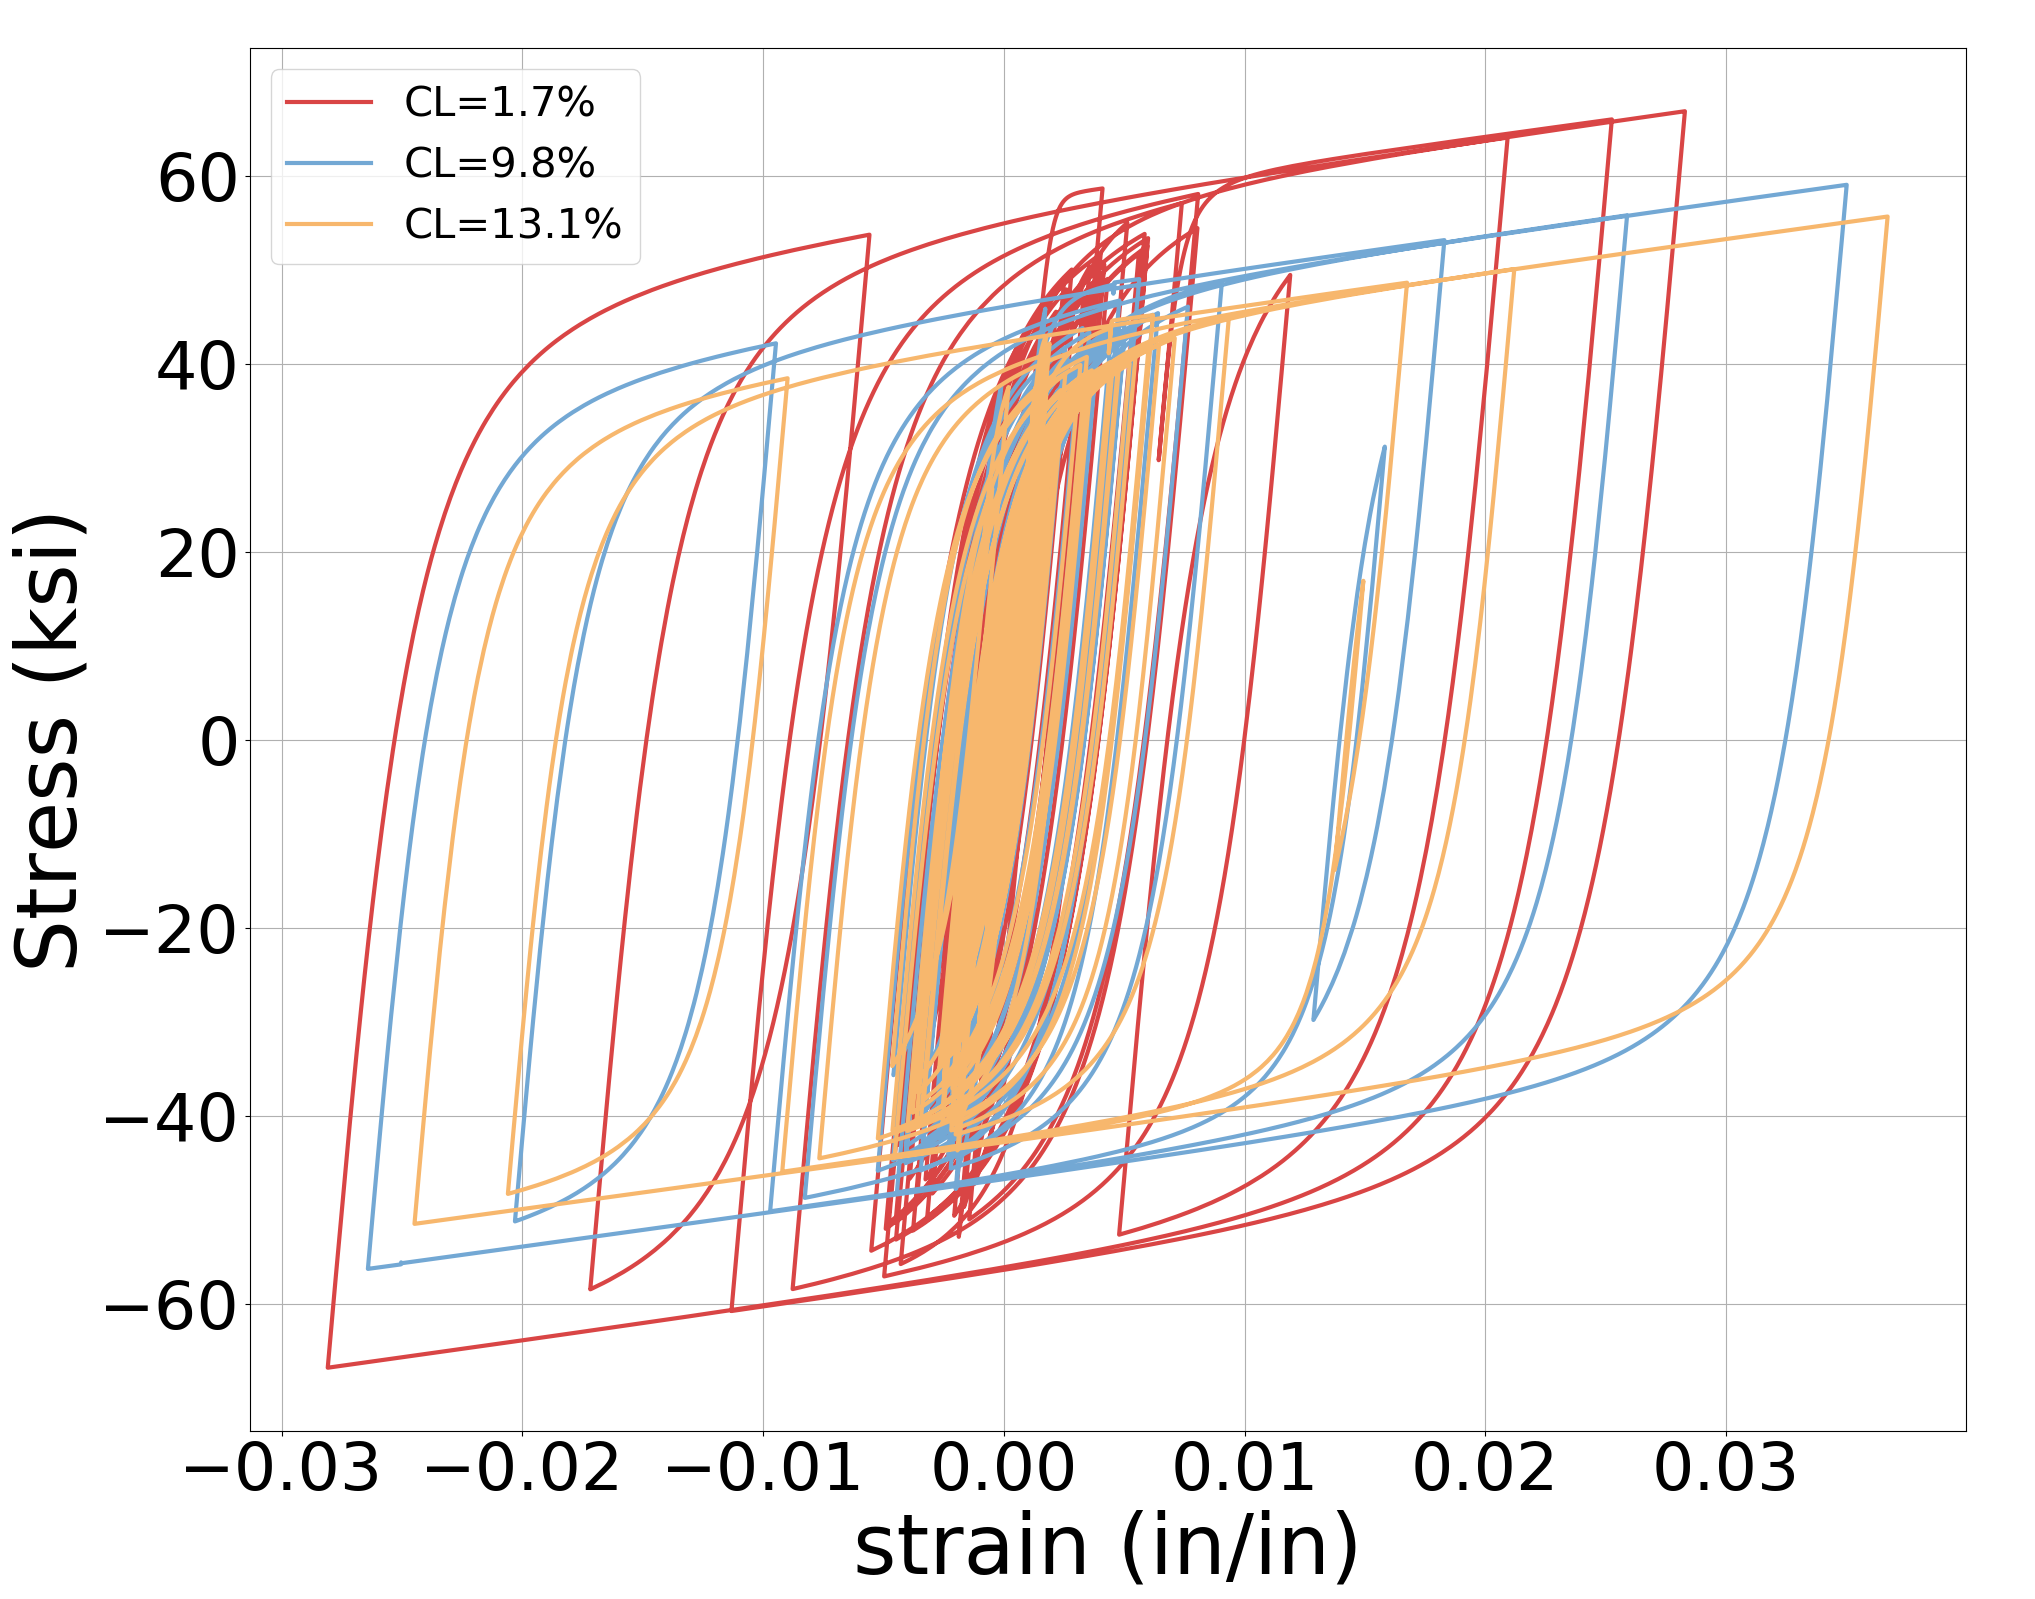
\includegraphics[width=0.65\textwidth]{Chapter-4/figs/Steel_StressStrain}
	\caption{Stress strain response for extreme rebar location}
	\label{fig:Steel_Stress_Strain_Response}
\end{figure}

\subsection{Development of cumulative distribution functions}

Once the analysis is complete the data is post-processed and expressed as a cumulative distribution function (CDF). The methodology employed corresponds to the multiple stripe analysis (MSA) recommended by Baker et al \cite{Baker2015}. While peak ground acceleration ($PGA$) has been widely used as the intensity measure to develop fragility functions\cite{Ghosh2015}\cite{Bisadi2015}\cite{Shekhar2018}, Krish \cite{Krish2018} in a recent study, showed that spectral displacement at first effective period ($IM=Sd(T_1)$) has better correlation than $PGA$. To demonstrate this, CDF curves were developed for $IM=PGA$ and $IM=Sd(T_1)$, and are shown in in figures \fref{fig:CDF_SY_PGA} and \fref{fig:CDF_SY_SDT1} correspondingly. The CDFs were developed for the steel yielding limit state, however this can be the extrapolated for any limit state. \fref{fig:CDF_SY_PGA} shows the results obtained with $IM=PGA$ do not show a good correlation since as corrosion increases the probability of exceeding a limit state decreases, this is not the behavior observed in \fref{fig:Steel_Stress_Strain_Response}. Conversely, \fref{fig:CDF_SY_SDT1} shows the results with $IM=Sd(T_1)$, these results present a better correlation, since, as corrosion increases, the probability of exceeding the limit state of yielding increases, for the preliminary results shown here the corrosion level of 13.1\% results are an exception. These results will improve as more analyses become available. 

\begin{figure}[htbp]
	\centering
	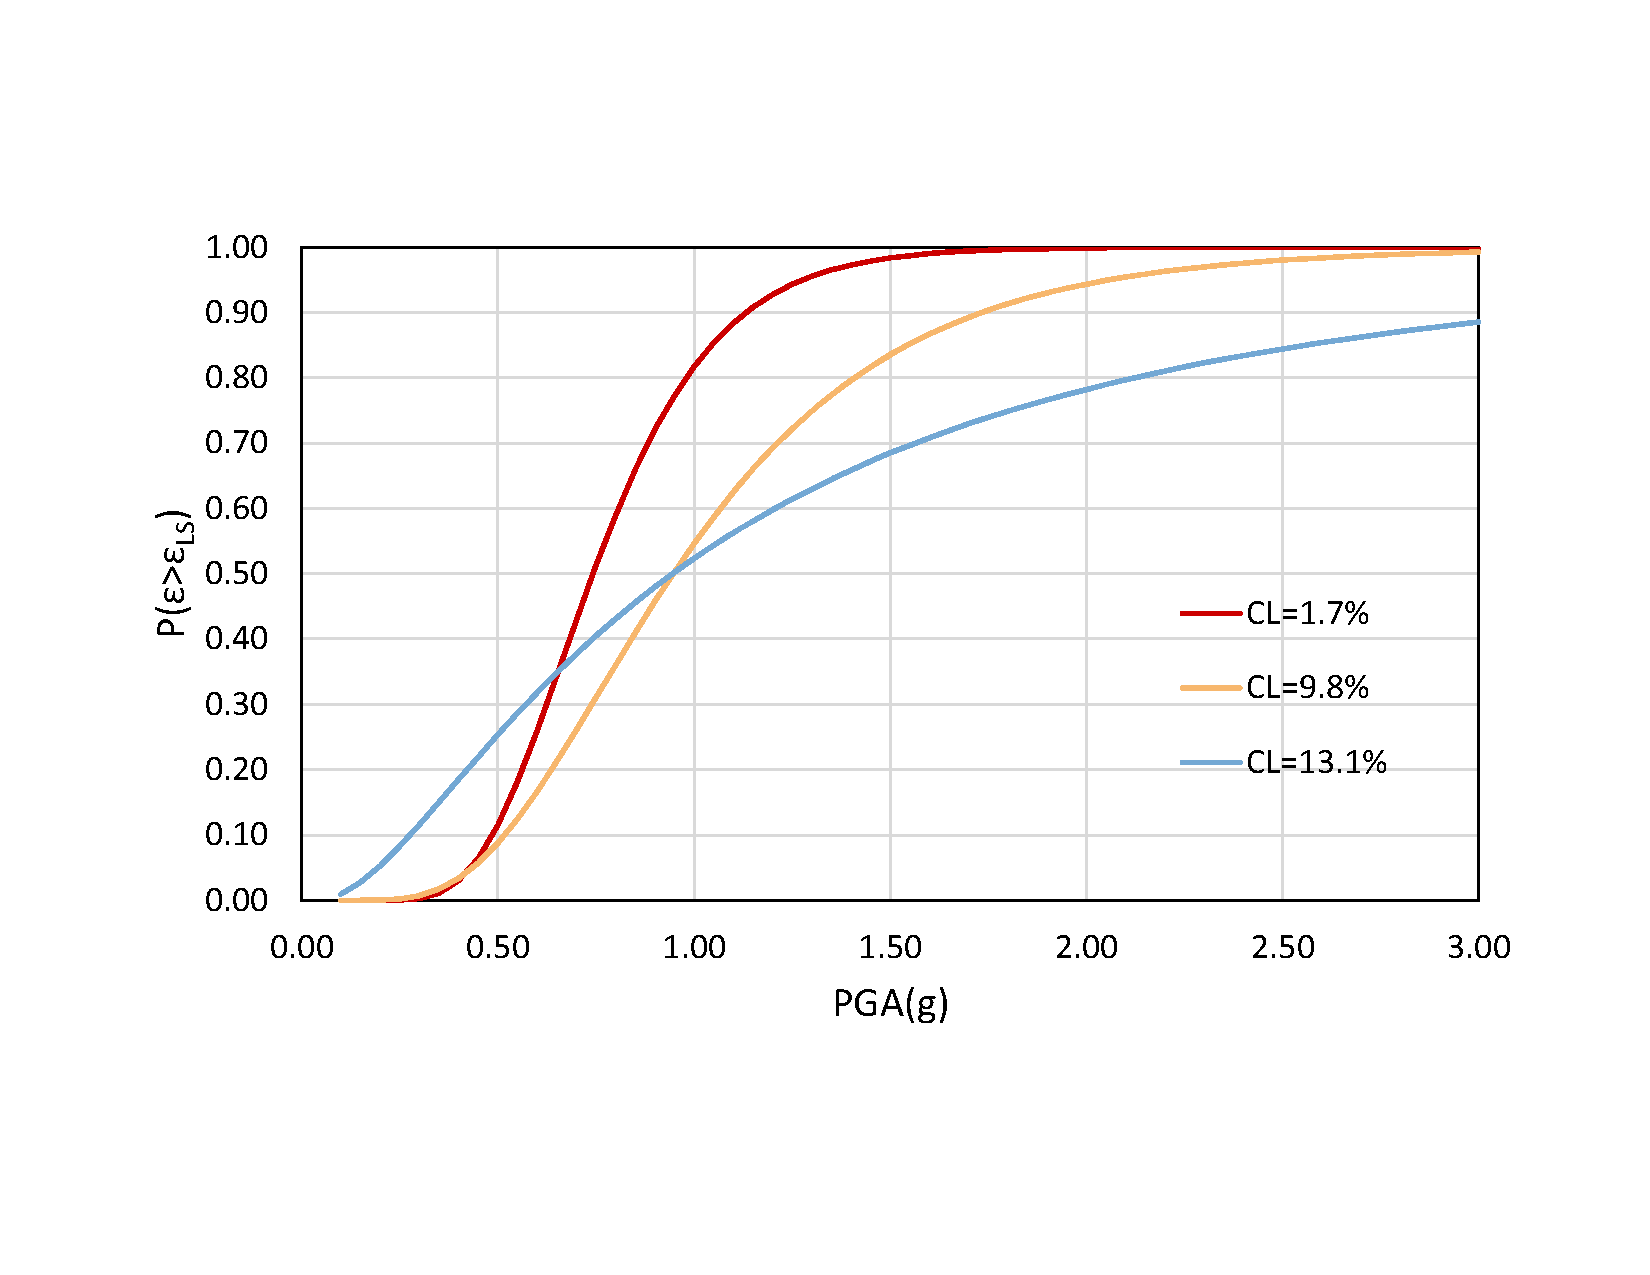
\includegraphics[width=0.8\textwidth]{Chapter-4/figs/CDF_PGA}
	\caption{CDF of steel yielding limit state using $IM=PGA$}
	\label{fig:CDF_SY_PGA}
\end{figure}
\begin{figure}[htbp]
	\centering
	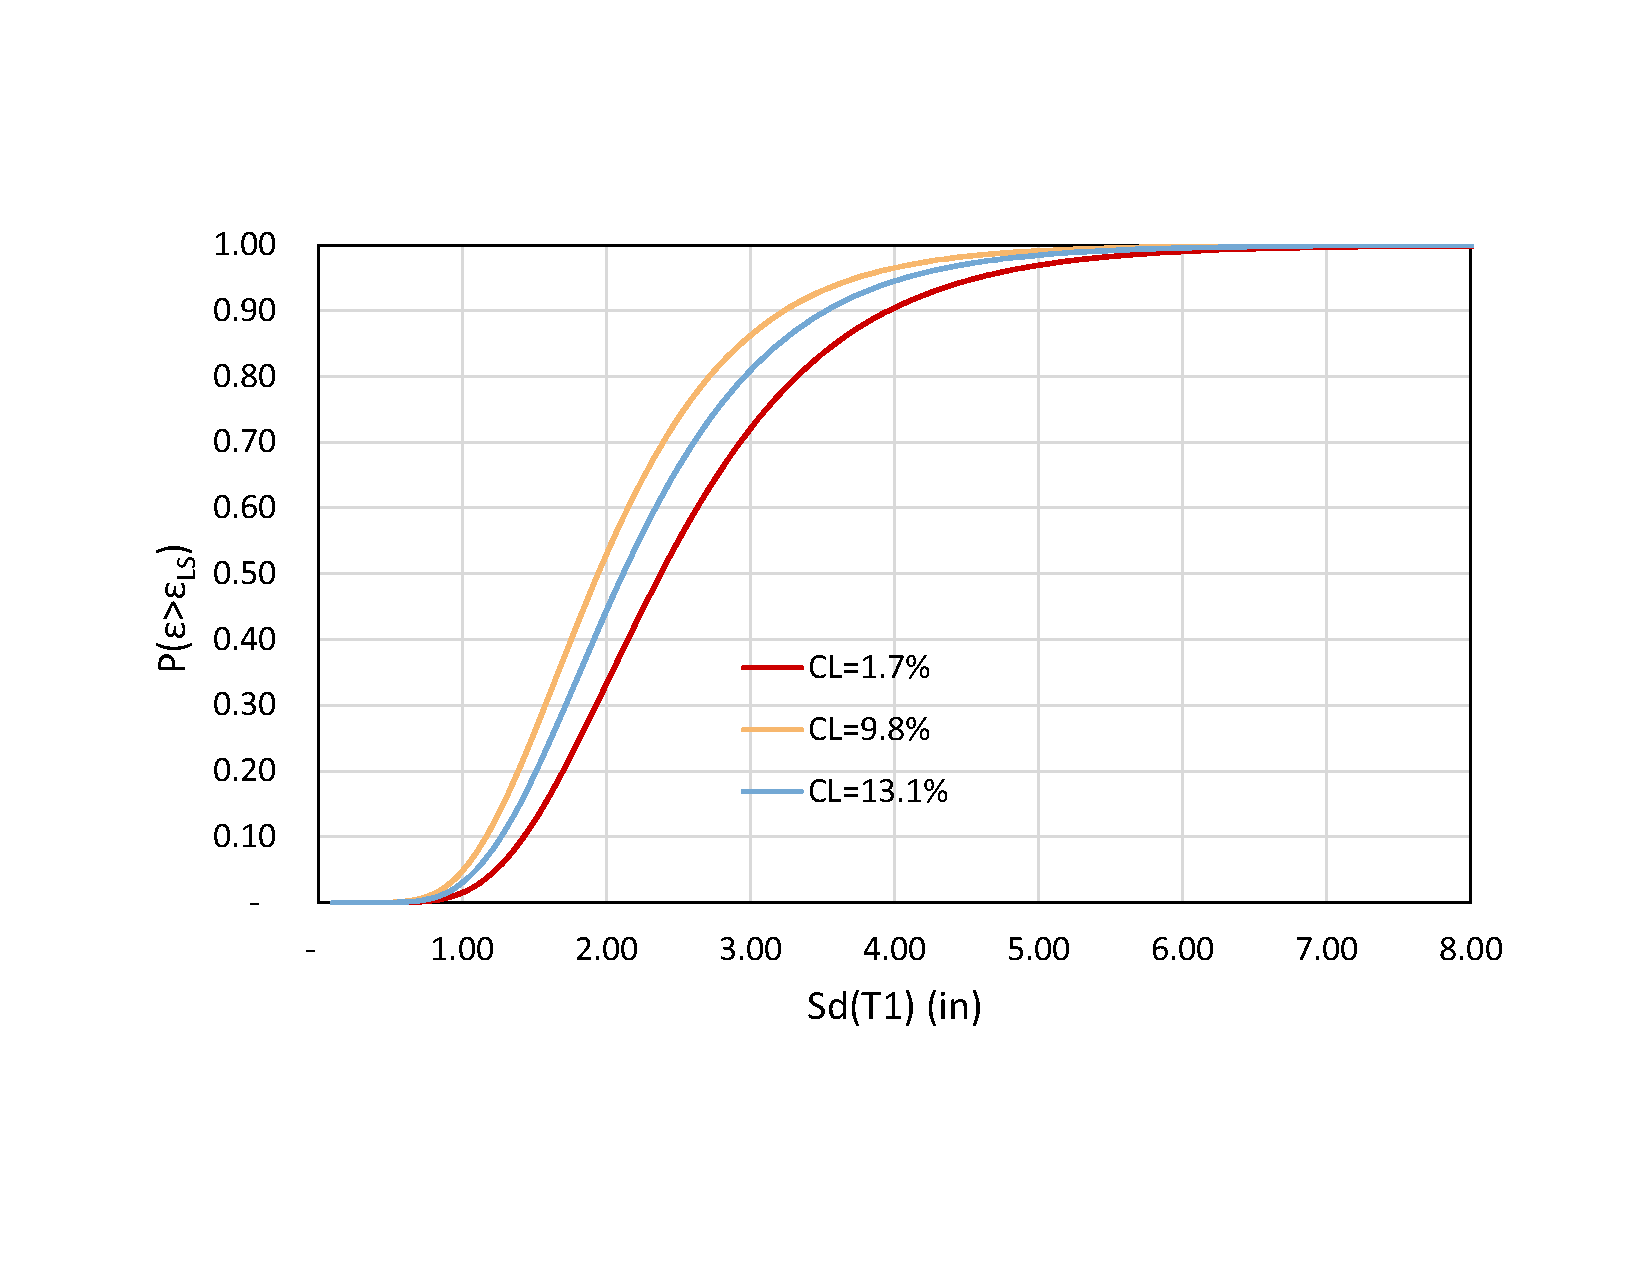
\includegraphics[width=0.8\textwidth]{Chapter-4/figs/CDF_SdT1}
	\caption{CDF of steel yielding limit state using $IM=Sd(T_1)$}
	\label{fig:CDF_SY_SDT1}
\end{figure}
\newpage
\subsection{Results discussion}
\begin{itemize}
	\item The results show that there is an increase in the demands as the corrosion in the structure increases. This is clearly shown in \fref{fig:CDF_SY_SDT1}. However, more results will help improve this correlation
	\item Results shown in \fref{fig:CDF_SY_PGA} and \fref{fig:CDF_SY_SDT1}, show that $IM=Sd(T_1)$ is a better intensity measure than $IM=PGA$
	\item The outcomes from the experimental campaign will further improve the results obtained in the analytical work
	\item The experimental phase will also provide an improved methodology to mimic the behavior of corroded reinforcing steel that is embedded inside the concrete
	\item The inclusion of additional aging conditions in the analysis will provide a realistic analysis of aging RC columns
\end{itemize}

\section{Future topics}

\begin{itemize}
	\item Concrete strength aging
	\item Welding and fatigue in steel structures
	\item Repair effects
	\item Main shock - after shock series - repair series
	\item Load history effects
	\item Degree of damage effect on confined structures behavior
	\item Selection of intensity measure (IM)
\end{itemize}
